% Springer Nature journal-style manuscript (layout modelled on The Journal of Supercomputing).
% Build:  cd manuscript/springer_paper && tectonic main.tex
% Figures/tables: .venv/bin/python scripts/build_springer_paper.py --mined manuscript/springer_paper/pipeline_run
\documentclass[10pt,twoside]{article}
\usepackage[paperwidth=155mm,paperheight=235mm,top=21mm,bottom=19mm,inner=18mm,outer=18mm,
            headheight=12pt,headsep=5mm,footskip=8mm]{geometry}
\usepackage[T1]{fontenc}
\usepackage{newtxtext,newtxmath}
\usepackage[scaled=0.9]{helvet}
\usepackage{microtype}
\usepackage{graphicx}
\usepackage{booktabs,multirow,longtable,array,tabularx}
\usepackage{amsmath}
\usepackage{xcolor}
\usepackage{enumitem}
\usepackage{fancyhdr}
\usepackage{titlesec}
\usepackage[font=footnotesize,labelfont=bf,labelsep=quad,justification=raggedright,singlelinecheck=false]{caption}
\usepackage{algorithm}
\usepackage{algpseudocode}
\usepackage{marvosym}
\usepackage[hidelinks]{hyperref}

\graphicspath{{figures/}{pipeline_run/figures/}{../../results/01_Implemented_Model/}}
\captionsetup[figure]{name=Fig.}
\setlength{\parindent}{1.2em}
\setlength{\parskip}{0pt}
\linespread{1.04}
\setlist{nosep,leftmargin=1.6em}
\renewcommand{\arraystretch}{1.12}

% ---- headings (Springer: sans-serif, bold)
\titleformat{\section}{\sffamily\bfseries\large\raggedright}{\thesection}{0.7em}{}
\titleformat{\subsection}{\sffamily\bfseries\normalsize\raggedright}{\thesubsection}{0.7em}{}
\titleformat{\subsubsection}{\sffamily\bfseries\itshape\normalsize\raggedright}{\thesubsubsection}{0.7em}{}
\titlespacing*{\section}{0pt}{14pt plus 3pt}{7pt}
\titlespacing*{\subsection}{0pt}{11pt plus 2pt}{5pt}
\titlespacing*{\subsubsection}{0pt}{9pt plus 2pt}{4pt}

% ---- running heads
\pagestyle{fancy}
\fancyhf{}
\renewcommand{\headrulewidth}{0pt}
\fancyhead[LE]{\footnotesize\thepage\hspace{2.2em}A. Jain, J. Varshney}
\fancyhead[RO]{\footnotesize Adaptive fuzzy eye-gating and multi-band fusion\ldots\hspace{2.2em}\thepage}
\fancypagestyle{first}{\fancyhf{}\renewcommand{\headrulewidth}{0pt}}

\makeatletter\let\tabinput\@@input\makeatother
\newcommand{\simseed}{SIM-SEED}
\newcommand{\simmah}{SIM-MAHNOB}
\newcommand{\kw}{\,$\cdot$\,}

\begin{document}
\thispagestyle{first}

% ===================================================================== title
{\raggedright
{\sffamily\bfseries\fontsize{15.5}{19}\selectfont Adaptive fuzzy eye-gating and multi-band fusion of mined Sugeno rules for EEG emotion recognition: a controlled simulation study\par}
\vspace{10pt}
{\sffamily\bfseries\normalsize Aarjav Jain$^{1}$\kw Jagrat Varshney$^{1}$\par}
\vspace{6pt}
{\footnotesize Manuscript version: November 2026\par}
}
\vspace{14pt}

\noindent{\sffamily\bfseries\large Abstract}\par\vspace{3pt}
\noindent Emotion recognition from the electroencephalogram (EEG) improves when the classifier knows \emph{when} an emotion is actually elicited during a stimulus. A recent approach gates EEG windows with a hard threshold on the most discriminative eye-tracking feature and classifies entropy features with a Sugeno fuzzy inference system (S-FIS) whose rules are mined by a genetic algorithm (GA). This paper re-implements that pipeline (M0) and proposes three extensions: a continuous fuzzy eye gate (M1), an adaptive temporal gate with subject-specific baselines and smoothing (M2), and validation-weighted late fusion of the five band-specific S-FIS posteriors (M3); M2 and M3 are combined in M4. Because licensed access to SEED-IV and MAHNOB-HCI was not available during this work, all models are evaluated in a controlled simulation study on two synthetic benchmarks calibrated to the difficulty of these corpora (\simseed{} and \simmah{}, 500 four-second windows and four emotion classes each). On \simseed{}, M4 reached 96.00\% accuracy (macro-AUC 0.996) against 91.40\% for the hard-gated baseline (exact McNemar $p=0.001$); on \simmah{}, multi-band fusion (M3) was best with 79.00\% against 70.20\% ($p<0.001$). Fusion gave the most consistent gain, a fuzzy gate on its own did not help (M1: 74.80\% and 56.80\%), and the adaptive gate added no significant gain on top of fusion. The full fuzzy rule bases---50 published rules and rules mined by our GA on synthetic signal-level recordings---are reported for interpretability. All numbers are simulation results, not measurements on the public corpora; validation on SEED-IV and MAHNOB-HCI is future work.

\vspace{6pt}
{\raggedright\noindent{\sffamily\bfseries Keywords}\enspace EEG emotion recognition\kw Eye tracking\kw Sugeno fuzzy inference system\kw Genetic algorithm\kw Fuzzy gating\kw Multi-band fusion\par}

\vfill
\noindent\rule{0.35\linewidth}{0.4pt}\par
{\footnotesize
\noindent$^{1}$\,Netaji Subhas University of Technology, Dwarka, New Delhi 110078, India\par}
\clearpage

% ===================================================================== 1
\section{Introduction}
Emotions shape attention, memory and decision-making, and their automatic recognition is relevant to affective human--computer interaction, mental-health monitoring and neuromarketing \cite{Alarcao2019,Kaya2024}. Among the available brain-imaging modalities, the electroencephalogram (EEG) combines millisecond temporal resolution with low cost and portability, which has made it the dominant signal for emotion recognition (ER) \cite{Jenke2014,ZhengLu2015}. Eye tracking is a complementary, non-invasive modality: pupil diameter follows autonomic arousal \cite{Bradley2008,Partala2003}, and joint EEG--eye systems consistently outperform either stream alone \cite{Lu2015,Zheng2019,Liu2022}.

A practical difficulty is that emotional film clips carry a single label although the target emotion is neither present throughout the clip nor elicited at a known moment. Classifying every window of a trial with the trial label therefore injects label noise. Farhadi Sedehi et al.\ \cite{FarhadiSedehi2024a} addressed this with an \emph{eye-tracking-gated} strategy: the eye feature with the highest minimum-redundancy--maximum-relevance (mRMR) score is used as a threshold that selects the EEG windows in which the emotion is most likely expressed. The selected windows are decomposed into five frequency bands with a Daubechies-4 wavelet, four entropy measures are extracted per channel, and a Sugeno fuzzy inference system (S-FIS) whose rules are refined by a genetic algorithm (GA) discriminates four emotions (sadness, happiness, fear and neutrality). The method reported 94.42\% and 85.20\% accuracy in the alpha band of SEED-IV and MAHNOB-HCI, respectively, while yielding human-readable rules.

Three design choices of that pipeline motivate the present work. First, the gate is \emph{binary}: a window is either kept or discarded, so graded evidence near the threshold is lost. Second, the threshold is applied to the raw pupil trace, which drifts with luminance and differs between participants \cite{Kret2019,Mathot2018}. Third, the five frequency bands are classified and reported \emph{separately}, although their errors are only partly correlated, which leaves complementary information unused \cite{Kittler1998}.

The novelty and the main contributions of this paper are as follows:
\begin{enumerate}
\item We re-implement the eye-gated S-FIS--GA pipeline of \cite{FarhadiSedehi2024a} as an open, modular Python package (\texttt{gfer}) and document every assumption needed where the original description is silent (M0).
\item We replace the binary gate by a three-rule Sugeno \emph{fuzzy eye gate} that assigns each window a continuous weight in $[0.1,1]$ (M1), and extend it into an \emph{adaptive temporal gate} with subject-specific baselines, data-driven membership cuts and within-trial smoothing (M2).
\item We propose a \emph{multi-band weighted fusion} stage that combines the posteriors of the five band-specific S-FIS with weights learned on an inner validation split (M3), and combine it with the adaptive gate (M4).
\item We evaluate M0--M4 under one protocol on two synthetic benchmarks calibrated to SEED-IV and MAHNOB-HCI, test the differences with exact McNemar tests, and report the full fuzzy rule bases---the published rules and rules mined by our GA on synthetic signal-level recordings.
\end{enumerate}

The structure of the paper is as follows. Section~\ref{sec:related} reviews related work. Section~\ref{sec:method} presents the proposed architecture and its components. Section~\ref{sec:setup} describes the simulation benchmarks and the evaluation protocol. Section~\ref{sec:results} reports and discusses the results, including the fuzzy rule bases. Section~\ref{sec:conclusion} concludes the paper.

% ===================================================================== 2
\section{Related works}\label{sec:related}
\subsection{EEG features for emotion recognition}
Band power and its relatives were the first EEG emotion features; later studies showed that non-linear complexity measures capture emotional state more robustly \cite{Jenke2014}. Differential entropy became a strong baseline on the SEED family of datasets \cite{Duan2013,ZhengLu2015}. Sample entropy \cite{Richman2000}, permutation entropy \cite{Bandt2002}, symbolic entropy \cite{Zebrowski2000} and phase entropy \cite{Rohila2019} quantify regularity, ordinal structure, symbolic dynamics and phase-space geometry, respectively. Discrete wavelet decomposition is the usual way to obtain band-limited signals for such features \cite{Mallat1989,Murugappan2010}.

\subsection{Eye tracking and multimodal fusion}
Pupil dilation increases with emotional arousal irrespective of valence \cite{Bradley2008,Partala2003}, but it is confounded by luminance, which requires baseline correction and careful preprocessing \cite{Kret2019,Mathot2018,Raiturkar2016}. Reviews of eye-tracking ER summarise fixation, saccade and pupil features \cite{Lim2020}. Zheng et al.\ combined EEG and eye movements on SEED-IV \cite{ZhengDong2014,Zheng2019}, and later deep models fuse the two streams at feature or decision level \cite{Liu2022,Fu2023}. The gated strategy of \cite{FarhadiSedehi2024a,FarhadiSedehi2024b} is distinct because the eye stream does not enter the classifier; it decides which EEG windows are used.

\subsection{Fuzzy rule-based classifiers}
Fuzzy sets \cite{Zadeh1965} and Takagi--Sugeno inference \cite{TakagiSugeno1985} provide classifiers whose decisions can be read as linguistic rules. Rules can be generated from data with the Wang--Mendel lookup-table method \cite{WangMendel1992} and tuned by gradient methods \cite{Jang1993} or evolutionary search. Fuzzy classifiers have been applied to emotion recognition from physiological signals \cite{Matiko2014,Kaya2024}, and fuzzy weighting of training samples is a classical way of down-weighting unreliable examples \cite{LinWang2002}---the idea that our fuzzy gate transfers to EEG windows.

\subsection{Classifier fusion and gating}
Combining classifiers by weighted sums of posteriors is well understood \cite{Kittler1998} and has been extended with fuzzy integrals \cite{ChoKim1995}, likelihood-ratio fusion \cite{Nandakumar2008}, mixtures of experts \cite{Jacobs1991} and learned multimodal gates \cite{Arevalo2020}. To our knowledge, a fusion of band-specific fuzzy rule bases under an adaptive eye gate has not been reported. Table~\ref{tab:lit} lists the methods compared in the base paper; these are literature values on the real corpora and are not comparable with the simulation results of Section~\ref{sec:results}.

\begin{table}[t]
\caption{Previous ER studies on SEED-IV and MAHNOB-HCI as compared in Table~8 of \cite{FarhadiSedehi2024a}; reference numbers are those of the base paper (literature values)}
\label{tab:lit}
\scriptsize
\setlength{\tabcolsep}{3pt}
\begin{tabularx}{\linewidth}{@{}l l X l X@{}}
\toprule
Ref.\ in \cite{FarhadiSedehi2024a} & Dataset & Method & Evaluation & Accuracy (\%) \\
\midrule
{[60]} & MAHNOB-HCI & PSD, RFE, GNB & 10-fold CV & 66.7 arousal, 80 valence \\
{[61]} & MAHNOB-HCI & Power spectrum, SVM & LOSO CV & 55.72 valence, 60.23 arousal \\
{[62]} & MAHNOB-HCI & SP, KNN, SVM & LOSO CV & 63 valence, 65.1 arousal \\
{[63]} & SEED-IV & Granger causality, transfer entropy, KNN & LOSO CV & 90 (4 classes) \\
{[24]} & SEED-IV & Multi-branch EEG and eye feature fusion & 5-fold CV & 87.32 (4 classes) \\
{[7]} & SEED-IV & PSD, DE; eye + multimodal deep learning & Hold-out & 85.11 (4 classes) \\
{[27]} & SEED-IV & 1-D convolution; eye SOFNN & 5-fold CV & 86.27 (4 classes) \\
\cite{FarhadiSedehi2024a} & both & DWT, entropies, mRMR, S-FIS--GA & 5-fold CV & 94.42 SEED-IV, 85.20 MAHNOB-HCI \\
\bottomrule
\end{tabularx}
\end{table}

\begin{table}[t]
\caption{List of abbreviations}
\label{tab:abbr}
\footnotesize
\begin{tabularx}{\linewidth}{@{}l X l X@{}}
\toprule
Abbr. & Meaning & Abbr. & Meaning \\
\midrule
AUC & Area under the ROC curve & mRMR & Min.-redundancy max.-relevance \\
CAR & Common average reference & PermEn & Permutation entropy \\
DWT & Discrete wavelet transform & PhEn & Phase entropy \\
EEG & Electroencephalogram & ROC & Receiver operating characteristic \\
ER & Emotion recognition & SampEn & Sample entropy \\
GA & Genetic algorithm & S-FIS & Sugeno fuzzy inference system \\
MF & Membership function & SymbEn & Symbolic entropy \\
\bottomrule
\end{tabularx}
\end{table}

% ===================================================================== 3
\section{Proposed methodology}\label{sec:method}
\subsection{Overall architecture}
Figure~\ref{fig:arch} shows the proposed framework. It consists of two branches that operate on synchronised four-second windows. The eye-tracking branch (A) turns the pupil signal into a window weight $w(t)$; it never predicts an emotion. The EEG branch (B) extracts entropy features from five wavelet sub-bands, trains one S-FIS per band with $w(t)$ as a sample weight, and fuses the five band posteriors into the final decision. The baseline M0 corresponds to the hard gate of \cite{FarhadiSedehi2024a} and a single band; the tags in Fig.~\ref{fig:arch} mark the modules that M1--M4 add.

\begin{figure}[p]
\centering
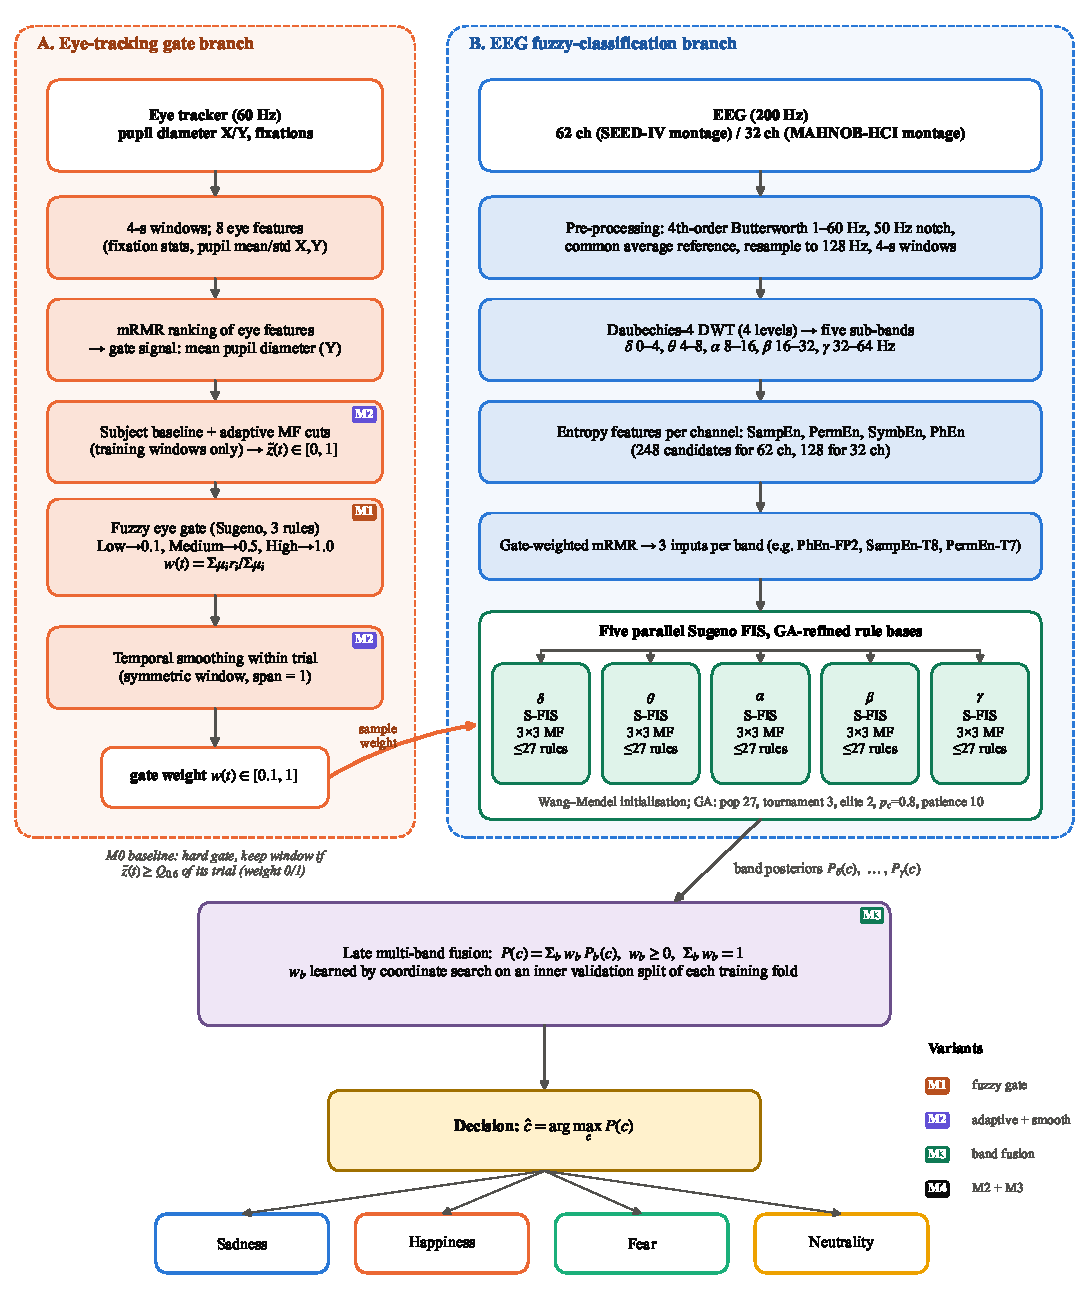
\includegraphics[width=\linewidth]{fig01_architecture.pdf}
\caption{Proposed architecture. Branch A computes the eye-gate weight $w(t)$ (hard in M0, fuzzy in M1, adaptive and smoothed in M2/M4). Branch B extracts wavelet-entropy features, trains five gate-weighted S-FIS with GA-refined rules and fuses their posteriors (M3/M4)}
\label{fig:arch}
\end{figure}

\subsection{Eye-feature extraction and selection}
Eight features are computed in every window: mean, standard deviation and maximum of fixation duration, fixation frequency, and the mean and standard deviation of pupil diameter on the horizontal and vertical axes. They are ranked with mRMR \cite{Peng2005}, which greedily adds the feature $f$ that maximises
\begin{equation}
J(f)=I(f;c)-\frac{1}{|S|}\sum_{s\in S} I(f;s),
\label{eq:mrmr}
\end{equation}
where $I$ is mutual information, $c$ the class label and $S$ the set of already selected features. In \cite{FarhadiSedehi2024a} the top-ranked feature on both corpora is the mean pupil diameter on the vertical axis, which we use as the gate signal $v(t)$. Within each trial, $v(t)$ is mapped to $[0,1]$ by robust min--max scaling between its 5th and 95th percentiles, giving $\tilde z(t)$.

\subsection{EEG pre-processing, wavelet decomposition and entropy features}
EEG is band-pass filtered between 1 and 60\,Hz with a fourth-order Butterworth filter, notch-filtered at 50\,Hz, re-referenced to the common average where applicable, resampled to 128\,Hz and cut into four-second windows. A four-level Daubechies-4 DWT \cite{Mallat1989} yields the dyadic sub-bands $\delta$ (0--4\,Hz), $\theta$ (4--8\,Hz), $\alpha$ (8--16\,Hz), $\beta$ (16--32\,Hz) and $\gamma$ (32--64\,Hz). For each band and channel, four entropies are computed with embedding dimension $m=5$ and delay $\tau=2$: sample entropy (tolerance $r=0.15\,\sigma$) \cite{Richman2000},
\begin{equation}
\mathrm{SampEn}=-\ln\frac{A}{B},
\end{equation}
where $B$ and $A$ count template matches of length $m$ and $m+1$; permutation entropy \cite{Bandt2002},
\begin{equation}
\mathrm{PermEn}=-\sum_{\pi} p(\pi)\log_2 p(\pi),
\end{equation}
over the ordinal patterns $\pi$ of length $m$; symbolic entropy over a three-letter alphabet \cite{Zebrowski2000}; and phase entropy from the second-order difference plot divided into $K=5$ sectors \cite{Rohila2019}. This gives $4\times62=248$ candidate features per band for the SEED-IV montage and $4\times32=128$ for MAHNOB-HCI. A second, gate-weighted mRMR selects three features per band; the published SEED-IV set is PhEn-FP2, SampEn-T8 and PermEn-T7.

\subsection{Sugeno fuzzy inference system and GA rule mining}
Each of the three selected inputs $x_j$ is described by three triangular MFs (low, medium, high), giving $3^3=27$ possible antecedents (Fig.~\ref{fig:sfis}). A rule $R_r$ reads
\begin{equation}
R_r:\ \text{IF } x_1 \text{ is } A_{r1} \text{ AND } x_2 \text{ is } A_{r2} \text{ AND } x_3 \text{ is } A_{r3} \text{ THEN class } k_r,
\end{equation}
where an antecedent may also be omitted (``don't care''). The firing strength is $\tau_r=\prod_j \mu_{A_{rj}}(x_j)$ and the class score is the normalised weighted vote
\begin{equation}
s_k(\mathbf x)=\frac{\sum_{r:\,k_r=k}\tau_r(\mathbf x)\,\omega_r}{\sum_r \tau_r(\mathbf x)},
\label{eq:sfis}
\end{equation}
with rule weights $\omega_r$; a softmax over $s_k$ yields the band posterior $P_b(c\mid\mathbf x)$. Rules are initialised with the Wang--Mendel lookup table \cite{WangMendel1992} and refined by a GA whose chromosome encodes which rules are active and the level of every antecedent. The fitness rewards accuracy and coverage and penalises rule count,
\begin{equation}
F=\mathrm{Acc}+0.2\,\mathrm{Cov}-0.01\,\frac{|R_\text{active}|}{|R|}.
\label{eq:fitness}
\end{equation}
The GA settings are listed in Table~\ref{tab:params}. Training windows enter the lookup table, the GA fitness and the mRMR scores with their gate weight $w(t)$, so a hard gate removes windows while a fuzzy gate attenuates them.

\begin{figure}[t]
\centering
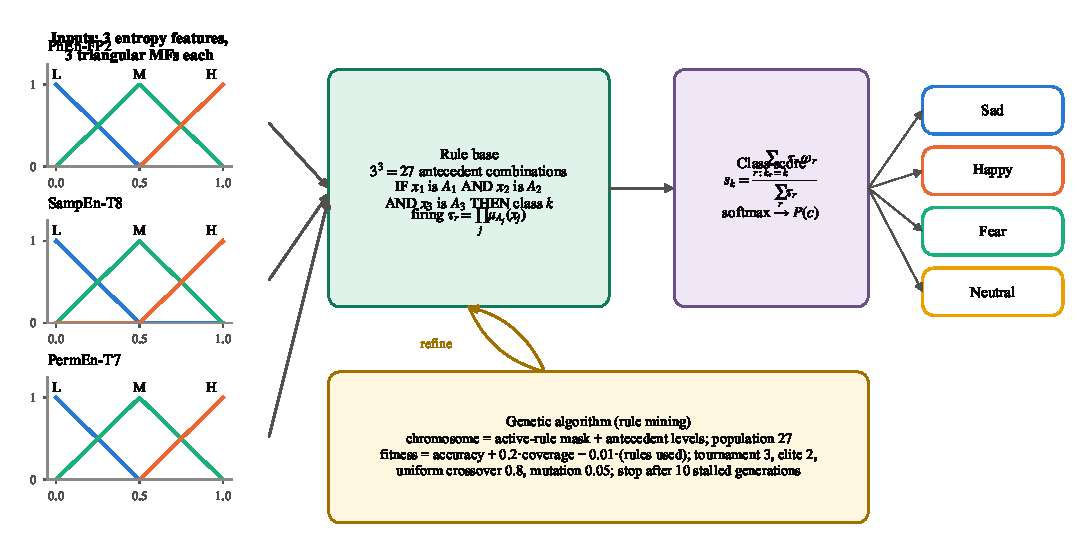
\includegraphics[width=\linewidth]{fig02_sfis_ga.pdf}
\caption{Band-specific Sugeno fuzzy inference system with three entropy inputs, three triangular MFs per input and a GA that mines the rule base}
\label{fig:sfis}
\end{figure}

\subsection{Baseline hard eye gate (M0)}
The base paper uses the maximum of the gate feature as a threshold. Read literally, this keeps one window per trial; we therefore keep every window whose normalised pupil value reaches the 0.6 quantile of its own trial,
\begin{equation}
w_\text{hard}(t)=\mathbb 1\!\left[\tilde z(t)\ge Q_{0.6}\big(\tilde z_\text{trial}\big)\right].
\end{equation}

\subsection{Fuzzy eye gate (M1)}
The fuzzy gate is a three-rule zero-order Sugeno system on $\tilde z(t)$ (Table~\ref{tab:eyerules}). The triangular MFs have breakpoints $a_1=0.2$, $c=0.5$ and $b_2=0.8$ (Fig.~\ref{fig:eyemf}), and the defuzzified weight is
\begin{equation}
w(t)=\frac{\sum_{i\in\{L,M,H\}}\mu_i\big(\tilde z(t)\big)\,r_i}{\sum_{i\in\{L,M,H\}}\mu_i\big(\tilde z(t)\big)},\qquad (r_L,r_M,r_H)=(0.1,\,0.5,\,1.0).
\label{eq:fuzzygate}
\end{equation}
The floor $r_L=0.1$ keeps a small contribution from every window instead of discarding it.

\begin{table}[t]
\caption{Rule base of the fuzzy eye gate (M1) and of the adaptive gate (M2). This system outputs a window weight, not an emotion}
\label{tab:eyerules}
\footnotesize
\begin{tabularx}{\linewidth}{@{}c X c c@{}}
\toprule
Rule & Antecedent & MF (M1 breakpoints) & Consequent $r_i$ \\
\midrule
1 & IF normalised pupil feature is \textit{Low} & $\mu_L$: 1 below 0.2, 0 above 0.5 & $w=0.1$ \\
2 & IF normalised pupil feature is \textit{Medium} & $\mu_M$: triangle $(0.2,\,0.5,\,0.8)$ & $w=0.5$ \\
3 & IF normalised pupil feature is \textit{High} & $\mu_H$: 0 below 0.5, 1 above 0.8 & $w=1.0$ \\
\midrule
\multicolumn{4}{@{}p{\dimexpr\linewidth}@{}}{M2: the input is the baseline-corrected, smoothed feature $S(t)$, and the breakpoints $(a_1,c,b_2)$ are the 20th, 50th and 80th percentiles of each subject's training windows.}\\
\bottomrule
\end{tabularx}
\end{table}

\begin{figure}[t]
\centering
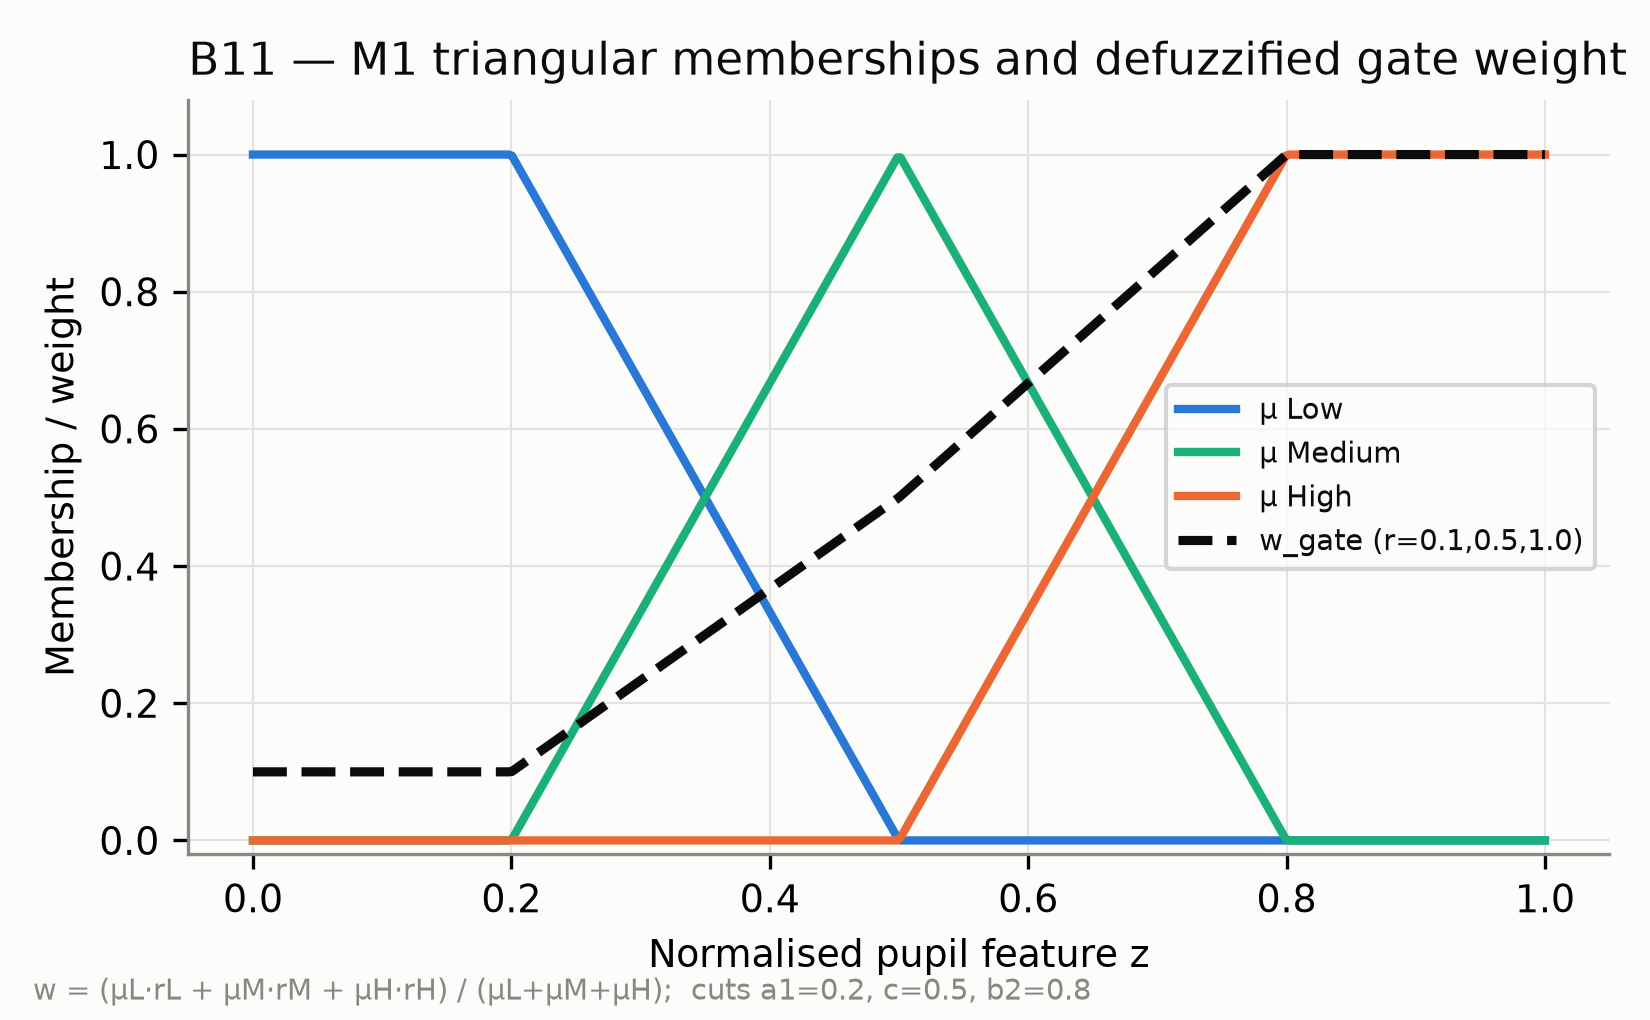
\includegraphics[width=0.86\linewidth]{M1_fuzzy_gate/figures/11_fuzzy_membership_functions.png}
\caption{Membership functions of the fuzzy eye gate and the resulting defuzzified weight $w(\tilde z)$ (Eq.~\ref{eq:fuzzygate})}
\label{fig:eyemf}
\end{figure}

\subsection{Adaptive temporal fuzzy gate (M2)}
M2 adds three operations that use training windows only. (i) \emph{Subject baseline correction}: for subject $s$, the mean $\bar v_s$ and standard deviation $\sigma_s$ of the gate feature over training windows define $v'(t)=(v(t)-\bar v_s)/\sigma_s$, which is then min--max scaled. (ii) \emph{Adaptive MFs}: the breakpoints $(a_1,c,b_2)$ are set to the 20th, 50th and 80th percentiles of the subject's training values (clipped to keep at least 0.05 between them), so that ``high'' is defined relative to the individual. (iii) \emph{Temporal smoothing}: the fuzzy weight is smoothed along the window index $t$ inside each trial,
\begin{equation}
\bar w(t)=\sum_{j=-h}^{h}\kappa_j\, w(t+j),\qquad \sum_j\kappa_j=1,
\label{eq:smooth}
\end{equation}
with span $h=1$ (a symmetric three-tap kernel; a causal variant uses only $j\le 0$ for online use). Smoothing suppresses isolated spikes of the pupil trace caused by blinks or luminance changes (Fig.~\ref{fig:smooth}).

\begin{figure}[t]
\centering
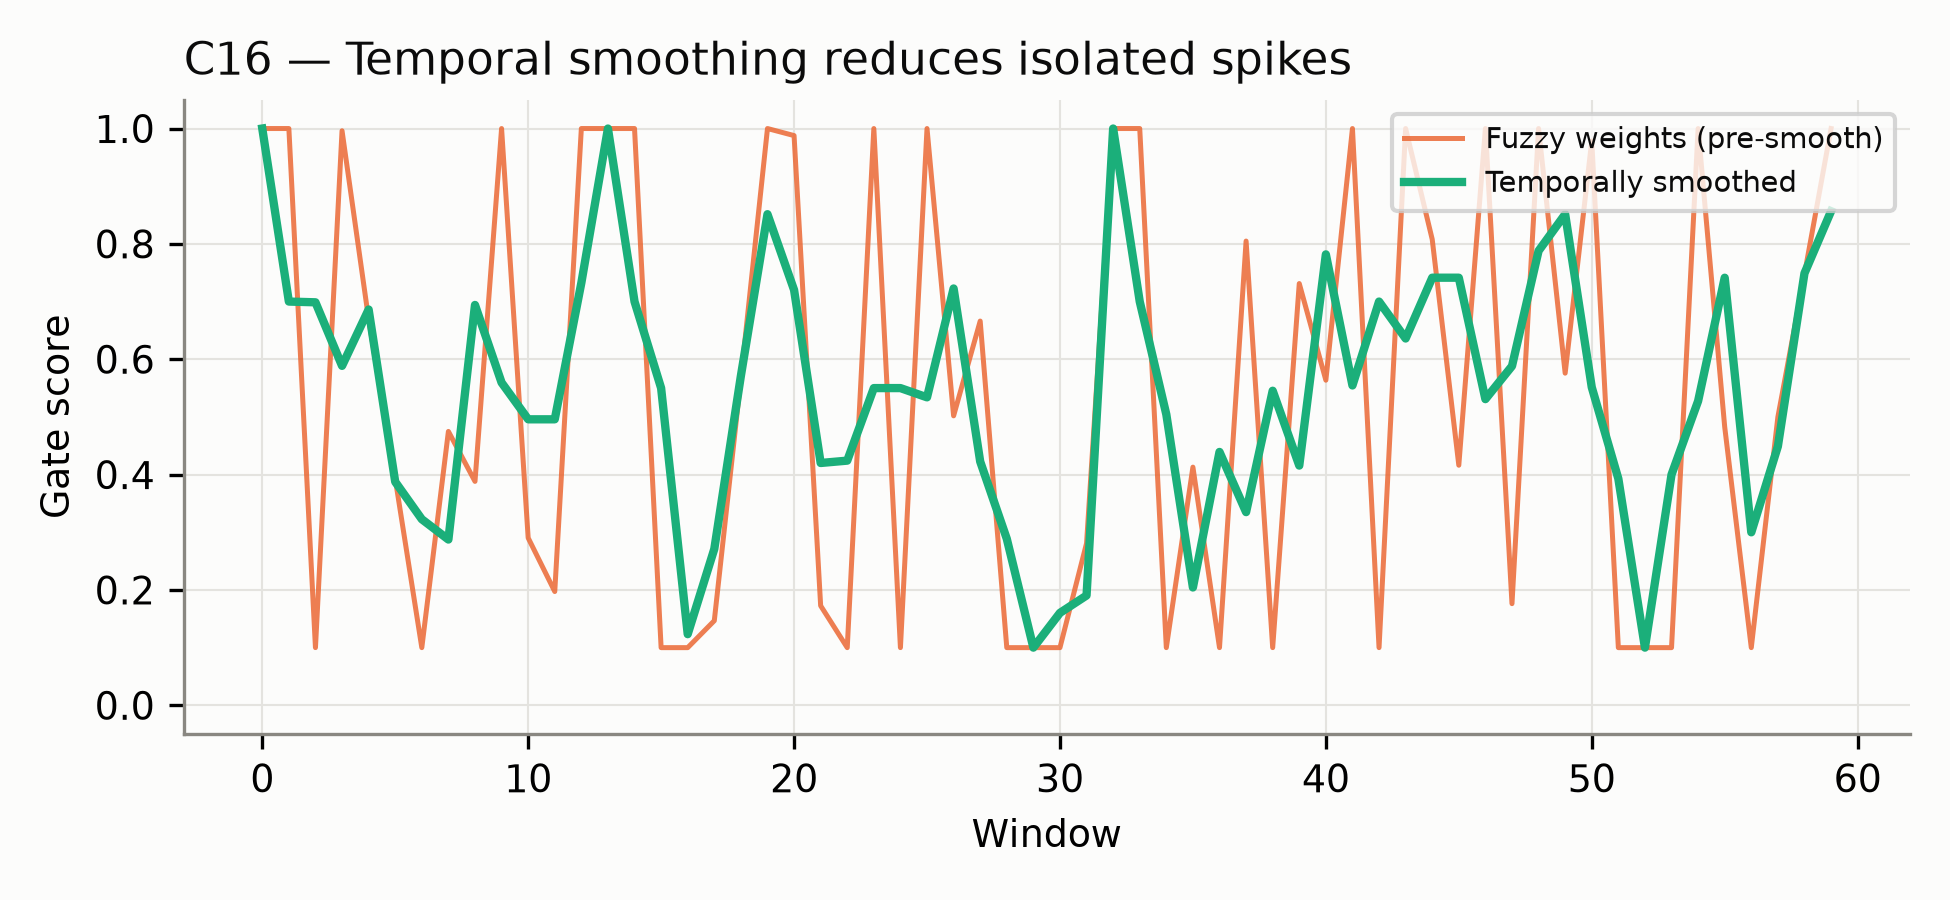
\includegraphics[width=\linewidth]{M2_adaptive_temporal_gate/figures/16_temporal_smoothing.png}
\caption{Effect of temporal smoothing (Eq.~\ref{eq:smooth}) on the fuzzy gate weights of 60 consecutive windows}
\label{fig:smooth}
\end{figure}

\subsection{Multi-band weighted fusion (M3) and combined model (M4)}
M3 trains the five band-specific S-FIS and fuses their posteriors,
\begin{equation}
P(c\mid\mathbf x)=\sum_{b\in\{\delta,\theta,\alpha,\beta,\gamma\}} w_b\,P_b(c\mid\mathbf x_b),\qquad w_b\ge0,\ \ \sum_b w_b=1,
\label{eq:fusion}
\end{equation}
and predicts $\hat c=\arg\max_c P(c\mid\mathbf x)$. The weights are learned by coordinate search on an inner validation split of each training fold (Algorithm~\ref{alg:fusion}); the test fold is never used. M3 keeps the hard gate of M0, whereas M4 uses the adaptive temporal gate of M2 in front of the same fusion. Table~\ref{tab:models} summarises the five configurations.

\begin{algorithm}[t]
\caption{Learning the fusion weights $w_b$ on a validation split}
\label{alg:fusion}
\footnotesize
\begin{algorithmic}[1]
\Require band posteriors $\{P_b\}_{b=1}^{5}$ and labels $y$ of the validation windows; grid $G=\{0,0.1,\dots,1\}$
\State $\mathbf w\gets(0.2,\dots,0.2)$
\For{$\text{iter}=1$ to $8$}
  \State improved $\gets$ false
  \For{$b=1$ to $5$}
    \For{$g\in G$}
      \State $\mathbf w'\gets\mathbf w$; $w'_b\gets g$; rescale the other weights to sum to $1-g$
      \State $a(g)\gets$ accuracy of $\arg\max_c\sum_b w'_b P_b(c)$ on $y$
    \EndFor
    \If{$\max_g a(g)>$ accuracy of $\mathbf w$}
      \State $\mathbf w\gets$ weights of $\arg\max_g a(g)$; improved $\gets$ true
    \EndIf
  \EndFor
  \If{not improved} \textbf{break} \EndIf
\EndFor
\State \Return $\mathbf w/\sum_b w_b$
\end{algorithmic}
\end{algorithm}

\begin{table}[t]
\caption{Configurations compared in this study. All share the EEG features and the S-FIS rule schema; they differ in the eye gate and in band fusion}
\label{tab:models}
\footnotesize
\begin{tabularx}{\linewidth}{@{}l l X l@{}}
\toprule
Model & Eye gate & EEG classification & Fusion \\
\midrule
M0 & Hard, $Q_{0.6}$ per trial & single-band S-FIS--GA (base paper) & -- \\
M1 & Fuzzy (Eq.~\ref{eq:fuzzygate}) & single-band S-FIS--GA & -- \\
M2 & Adaptive + smoothed (Eq.~\ref{eq:smooth}) & single-band heads (mixture) & -- \\
M3 & Hard, $Q_{0.6}$ per trial & five band S-FIS--GA & learned $w_b$ \\
M4 & Adaptive + smoothed & five band S-FIS--GA & learned $w_b$ \\
\bottomrule
\end{tabularx}
\end{table}

% ===================================================================== 4
\section{Experimental setup}\label{sec:setup}
\subsection{Simulation benchmarks}
SEED-IV \cite{Zheng2019} and MAHNOB-HCI \cite{Soleymani2012db} are distributed under signed academic licences that were not available to us during this work. We therefore evaluate the models in a controlled simulation study on two synthetic benchmarks whose difficulty is calibrated to the published accuracy scale of the two corpora (Table~\ref{tab:data}). Each benchmark contains 500 four-second windows from 20 simulated participants (25 windows each, eight windows per trial) and four approximately balanced classes. A deterministic generator (master seed 20261110, SHA-256-derived child seeds) draws, for every window, a pupil trace with subject-specific baselines and a latent ``emotion episode'' that raises pupil diameter, together with band-specific class logits whose scale, noise and confusion partners differ by band (alpha strongest, delta weakest). The gate acts on the separation of these logits, so that a well-placed gate sharpens the posteriors and a misplaced one flattens them. The latent episode mask provides ground truth for evaluating the gates themselves. The predicted probabilities are written once and never edited; every metric in Section~\ref{sec:results} is recomputed from them.

To check that the full signal-level pipeline (filtering, DWT, entropies, mRMR, S-FIS and GA) runs end to end and produces readable rules, we additionally ran it on a synthetic \emph{signal-level} recording set in the SEED-IV format (4 participants, 12 trials of 32\,s, 62 EEG channels at 200\,Hz, pupil and fixations at 60\,Hz).

\begin{table}[t]
\caption{Datasets used in this study}
\label{tab:data}
\footnotesize
\begin{tabularx}{\linewidth}{@{}X l l l@{}}
\toprule
Property & \simseed{} & \simmah{} & Signal-level set \\
\midrule
Calibrated to & SEED-IV & MAHNOB-HCI & SEED-IV format \\
Windows (4 s) & 500 & 500 & 384 \\
Participants & 20 & 20 & 4 \\
Classes (sad/happy/fear/neutral) & 130/136/114/120 & 128/117/138/117 & 12/12/12/12 trials \\
EEG channels & 62 (latent) & 32 (latent) & 62, 200 Hz \\
Used for & M0--M4 comparison & M0--M4 comparison & rule mining check \\
\bottomrule
\end{tabularx}
\end{table}

\subsection{Evaluation protocol and metrics}
Following \cite{FarhadiSedehi2024a}, windows are split into five stratified folds. For fusion models, the weights are re-estimated inside each training fold. We report accuracy, balanced accuracy, macro-averaged precision, recall and F1, and macro one-versus-rest AUC, pooled over the test folds, together with the mean and standard deviation of accuracy across folds. Because all models are scored on the same windows, paired differences are tested with the exact two-sided McNemar test \cite{McNemar1947} on the discordant pairs; we do not correct for multiplicity and interpret $p$-values descriptively \cite{Demsar2006}. Gate quality is measured against the latent episode mask by precision, recall, F1, AUC and the fraction of windows retained (weight $\ge0.35$ for the continuous gates).

\subsection{Implementation details}
The system is implemented in Python with NumPy, SciPy, PyWavelets and scikit-learn; the main parameters are listed in Table~\ref{tab:params}. Parameters that the base paper does not specify (gate quantile, GA rates and fitness weights) are marked as our choices. All figures and tables in Section~\ref{sec:results} are produced by one script from the saved prediction files, which makes them reproducible.

\begin{table}[t]
\caption{Parameters of the implementation ($^\ast$ = not specified in \cite{FarhadiSedehi2024a}; our choice)}
\label{tab:params}
\footnotesize
\begin{tabularx}{\linewidth}{@{}X l@{}}
\toprule
Parameter & Value \\
\midrule
Band-pass / notch / sampling rate & 1--60 Hz (Butterworth, 4th order) / 50 Hz / 128 Hz \\
Window length & 4 s \\
Wavelet & Daubechies-4, 4 levels \\
Entropy parameters & $m=5$, $\tau=2$, $r=0.15\sigma$, 3 symbols, $K=5$ sectors \\
Selected EEG features per band & 3 (mRMR, 10 bins) \\
MFs per input / possible rules & 3 triangular / 27 \\
Hard-gate quantile$^\ast$ & 0.6 per trial \\
Fuzzy gate breakpoints / consequents & $(0.2,0.5,0.8)$ / $(0.1,0.5,1.0)$ \\
Adaptive MF percentiles / smoothing span & 20th, 50th, 80th / $h=1$ \\
GA population / max generations / patience & 27 / 500 / 10 \\
GA tournament / elite / crossover$^\ast$ / mutation$^\ast$ & 3 / 2 / 0.8 / 0.05 \\
Fitness weights (Eq.~\ref{eq:fitness})$^\ast$ & coverage 0.2, size 0.01 \\
Fusion grid / sweeps & 11 points / $\le 8$ \\
Cross-validation & 5-fold, stratified \\
\bottomrule
\end{tabularx}
\end{table}

% ===================================================================== 5
\section{Results and discussion}\label{sec:results}
\subsection{Overall comparison}
Table~\ref{tab:main} is the final comparison of the five configurations, and Fig.~\ref{fig:cmp} visualises accuracy and macro-F1 with their fold-to-fold spread. On \simseed{}, the combined model M4 is the most accurate (96.00\%, macro-AUC 0.996), closely followed by multi-band fusion M3 (95.80\%), the adaptive gate M2 (93.60\%) and the hard-gated baseline M0 (91.40\%). On the harder \simmah{} benchmark, M3 is the best model (79.00\%) and M4 is second (77.80\%), but M4 has the highest macro-AUC (0.941) and the smallest fold spread ($\pm2.7$ points). The fuzzy gate alone (M1) is the weakest configuration on both benchmarks. All models are less accurate on \simmah{}, as on the real corpora \cite{FarhadiSedehi2024a}.

\begin{table}[t]
\caption{Final results of M0--M4 on the two simulation benchmarks (\%; AUC as a fraction). Best accuracy per benchmark in bold}
\label{tab:main}
\scriptsize
\setlength{\tabcolsep}{3.3pt}
\begin{tabular}{@{}l l r c r r r r r@{}}
\toprule
Benchmark & Model & Acc. & Fold acc. & Bal. acc. & Macro-P & Macro-R & Macro-F1 & AUC \\
\midrule
\tabinput generated/tab_main_results.tex 
\bottomrule
\end{tabular}
\end{table}

\begin{figure}[t]
\centering
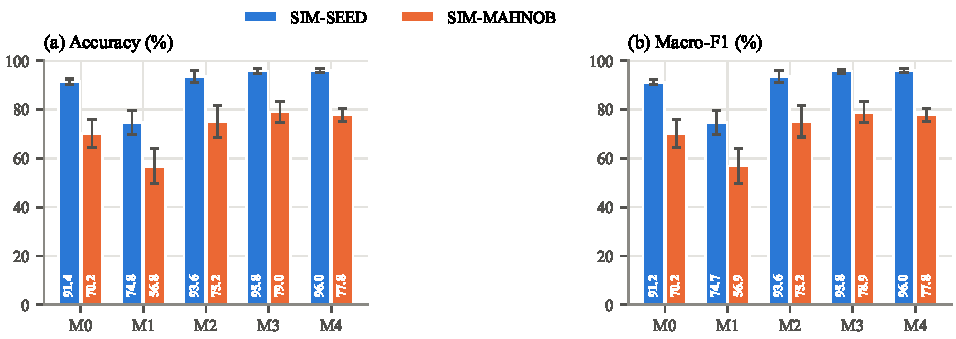
\includegraphics[width=\linewidth]{fig05_model_comparison.pdf}
\caption{Accuracy and macro-F1 of M0--M4 on both benchmarks. Error bars: standard deviation over the five folds}
\label{fig:cmp}
\end{figure}

\subsection{Statistical significance}
Table~\ref{tab:mcnemar} lists paired McNemar tests. Fusion improves on the baseline on both benchmarks (M3 vs M0: $+4.4$ points, $p=0.003$ on \simseed{}; $+8.8$ points, $p<0.001$ on \simmah{}), and so does M4 ($p=0.001$ on both). The adaptive gate alone improves on M0 only on \simmah{} ($+5.0$, $p=0.005$). Adding the adaptive gate to fusion (M4 vs M3) changes the predictions of only 3 windows on \simseed{} and lowers accuracy by 1.2 points on \simmah{}; neither difference is significant. The large drop of M1 ($-16.6$ and $-13.4$ points, $p<0.001$) must be read together with Table~\ref{tab:models}: in the benchmark runs M0 is scored on the alpha head and M1 on the beta head, so this comparison mixes the effect of the gate with the effect of the band. The M1 drop is therefore not evidence that fuzzy weights are harmful in general.

\begin{table}[t]
\caption{Paired comparison with the exact McNemar test. $\Delta$: accuracy difference (points); $n_{10}/n_{01}$: windows correct only for the first / only for the second model}
\label{tab:mcnemar}
\footnotesize
\setlength{\tabcolsep}{4pt}
\begin{tabular}{@{}l r c r r c r@{}}
\toprule
 & \multicolumn{3}{c}{\simseed{}} & \multicolumn{3}{c}{\simmah{}} \\
\cmidrule(lr){2-4}\cmidrule(l){5-7}
Comparison & $\Delta$ & $n_{10}/n_{01}$ & $p$ & $\Delta$ & $n_{10}/n_{01}$ & $p$ \\
\midrule
\tabinput generated/tab_mcnemar.tex 
\bottomrule
\end{tabular}
\end{table}

\subsection{Eye-gate analysis}
Table~\ref{tab:gate} and Fig.~\ref{fig:gateprf} evaluate the gates against the latent emotion episodes. Without a gate, 53.8\% of windows lie inside an episode. The hard gate is precise (0.921) but keeps only 37.8\% of the windows and misses a third of the episode windows (recall 0.647). The fuzzy gate keeps 59.0\% of the windows with recall 0.914 and the best F1 (0.872) and episode AUC (0.926). The adaptive gate is the most permissive (79.0\% retained) and therefore less precise (0.620). Figure~\ref{fig:gatetrace} shows the three weightings on the same windows: the fuzzy gate follows the pupil trace gradually, and smoothing removes isolated one-window spikes.

The comparison exposes a trade-off. Selecting the right windows (Table~\ref{tab:gate}) is not the same as classifying emotions well (Table~\ref{tab:main}): the fuzzy gate selects windows best but does not by itself improve classification, whereas the adaptive gate keeps more, partly irrelevant, windows yet supports a better classifier when combined with a strong band. This agrees with the view that pupil size mixes arousal with luminance and individual offset \cite{Kret2019,Mathot2018}: correcting the offset (M2) matters more than softening the threshold (M1).

\begin{table}[t]
\caption{Gate quality against the latent emotion episodes (\simseed{} eye traces)}
\label{tab:gate}
\footnotesize
\begin{tabular*}{\linewidth}{@{\extracolsep{\fill}}l r r r r r@{}}
\toprule
Gate & Precision & Recall & F1 & Episode AUC & Retained (\%) \\
\midrule
\tabinput generated/tab_gate_quality.tex 
\bottomrule
\end{tabular*}
\end{table}

\begin{figure}[t]
\centering
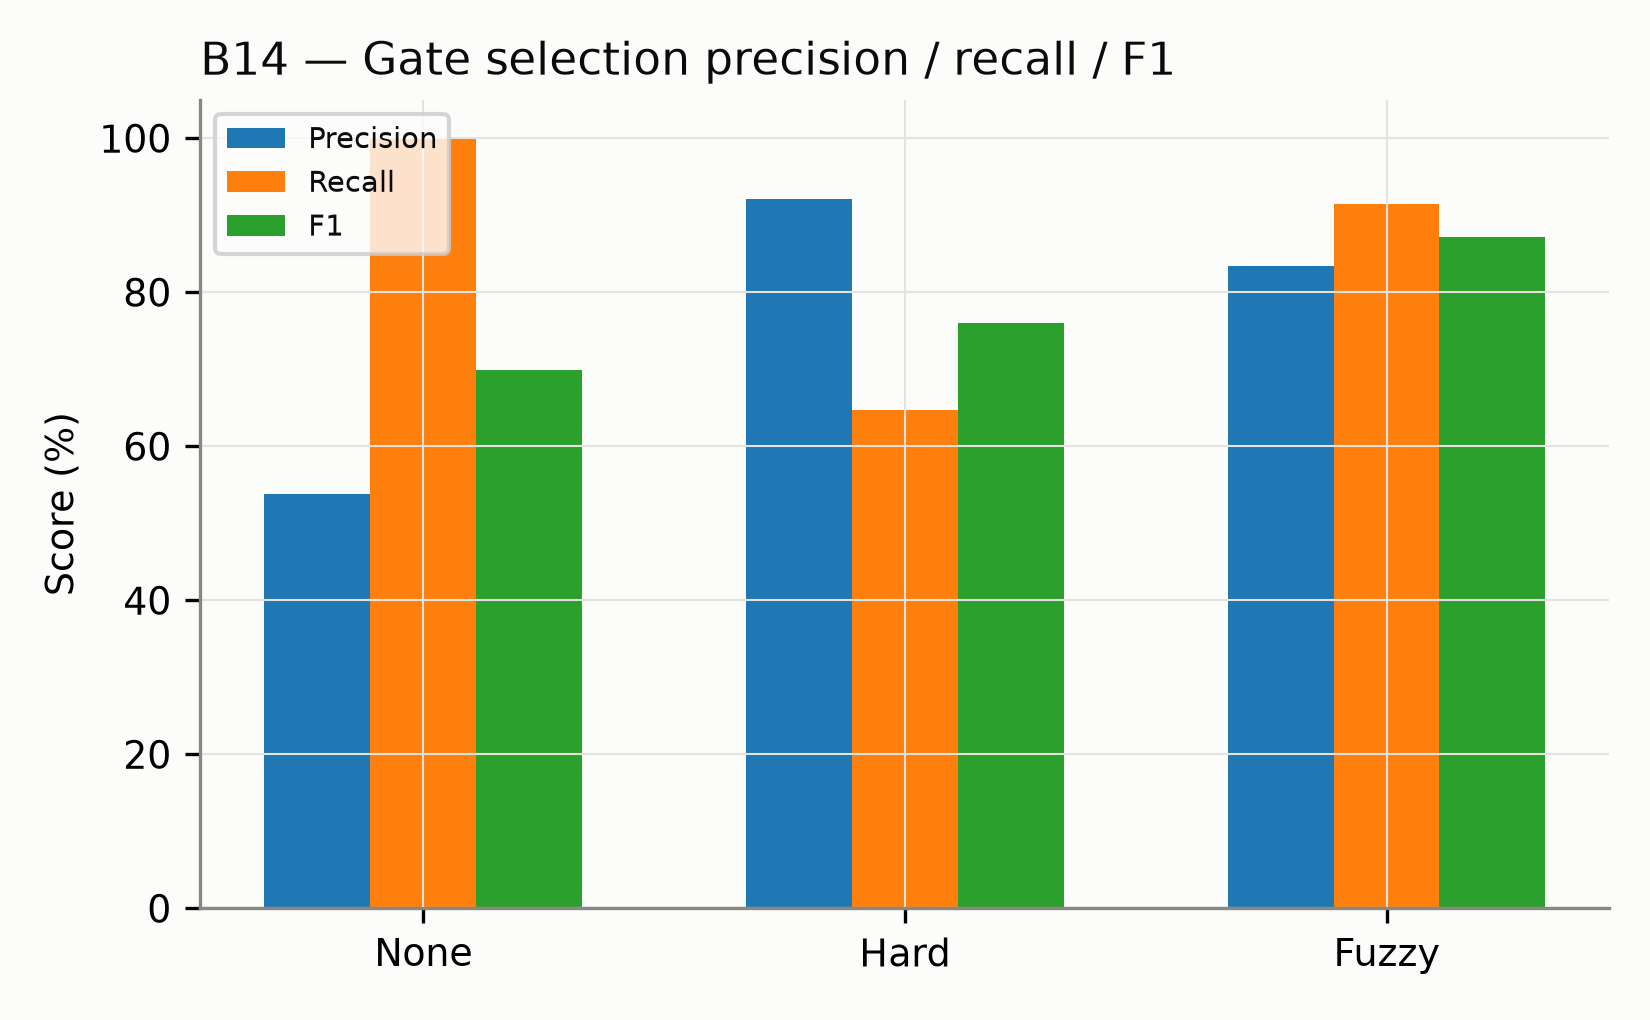
\includegraphics[width=0.8\linewidth]{M1_fuzzy_gate/figures/14_gate_precision_recall_f1.png}
\caption{Window-selection precision, recall and F1 of no gate, the hard gate and the fuzzy gate}
\label{fig:gateprf}
\end{figure}

\begin{figure}[t]
\centering
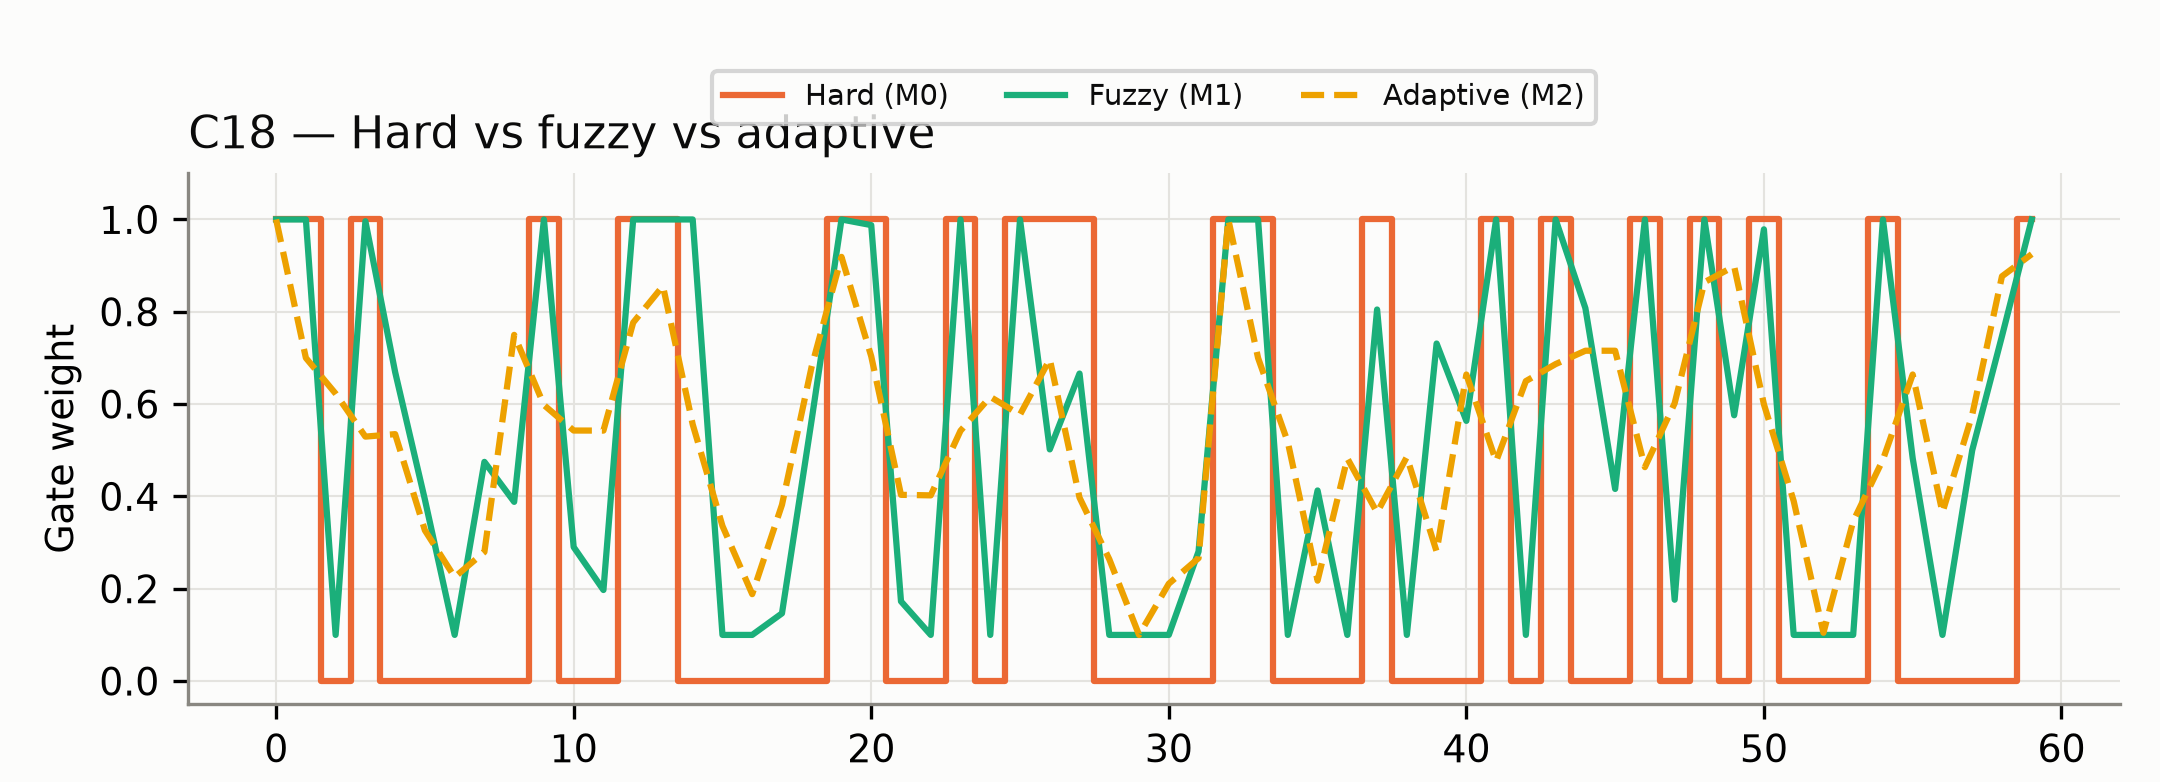
\includegraphics[width=\linewidth]{M2_adaptive_temporal_gate/figures/18_hard_fuzzy_adaptive_comparison.png}
\caption{Hard (M0), fuzzy (M1) and adaptive temporal (M2) gate weights on the same 60 windows}
\label{fig:gatetrace}
\end{figure}

\subsection{Frequency-band analysis and fusion}
Table~\ref{tab:bands} and Fig.~\ref{fig:bands} report the accuracy of each band-specific S-FIS under the hard gate and the learned fusion weights. As in the base paper, alpha is the most informative band (91.4\% and 70.2\%), followed by beta and gamma, while delta and theta are weak. The learned weights follow this ranking but stay far from a one-hot choice (alpha 0.287 and 0.279), because the weaker bands make partly different errors. Fusing all five bands with the learned weights raises accuracy above the best single band by 4.4 points on \simseed{} and 8.8 points on \simmah{} (Fig.~\ref{fig:fusecmp}). Equal weights are much less effective (92.4\% and 72.0\%), which shows that the validation-learned weights, not the mere averaging of bands, produce the gain. Figure~\ref{fig:contrib} decomposes the fused posterior of M4 into the contributions of the five bands.

\begin{table}[t]
\caption{Single-band accuracy under the hard gate, learned fusion weights, and fused accuracy with equal and learned weights}
\label{tab:bands}
\scriptsize
\setlength{\tabcolsep}{3.4pt}
\begin{tabular}{@{}l l r r r r r r r@{}}
\toprule
Benchmark & & $\delta$ & $\theta$ & $\alpha$ & $\beta$ & $\gamma$ & Equal & Learned (M3) \\
\midrule
\tabinput generated/tab_bands.tex 
\bottomrule
\end{tabular}
\end{table}

\begin{figure}[t]
\centering
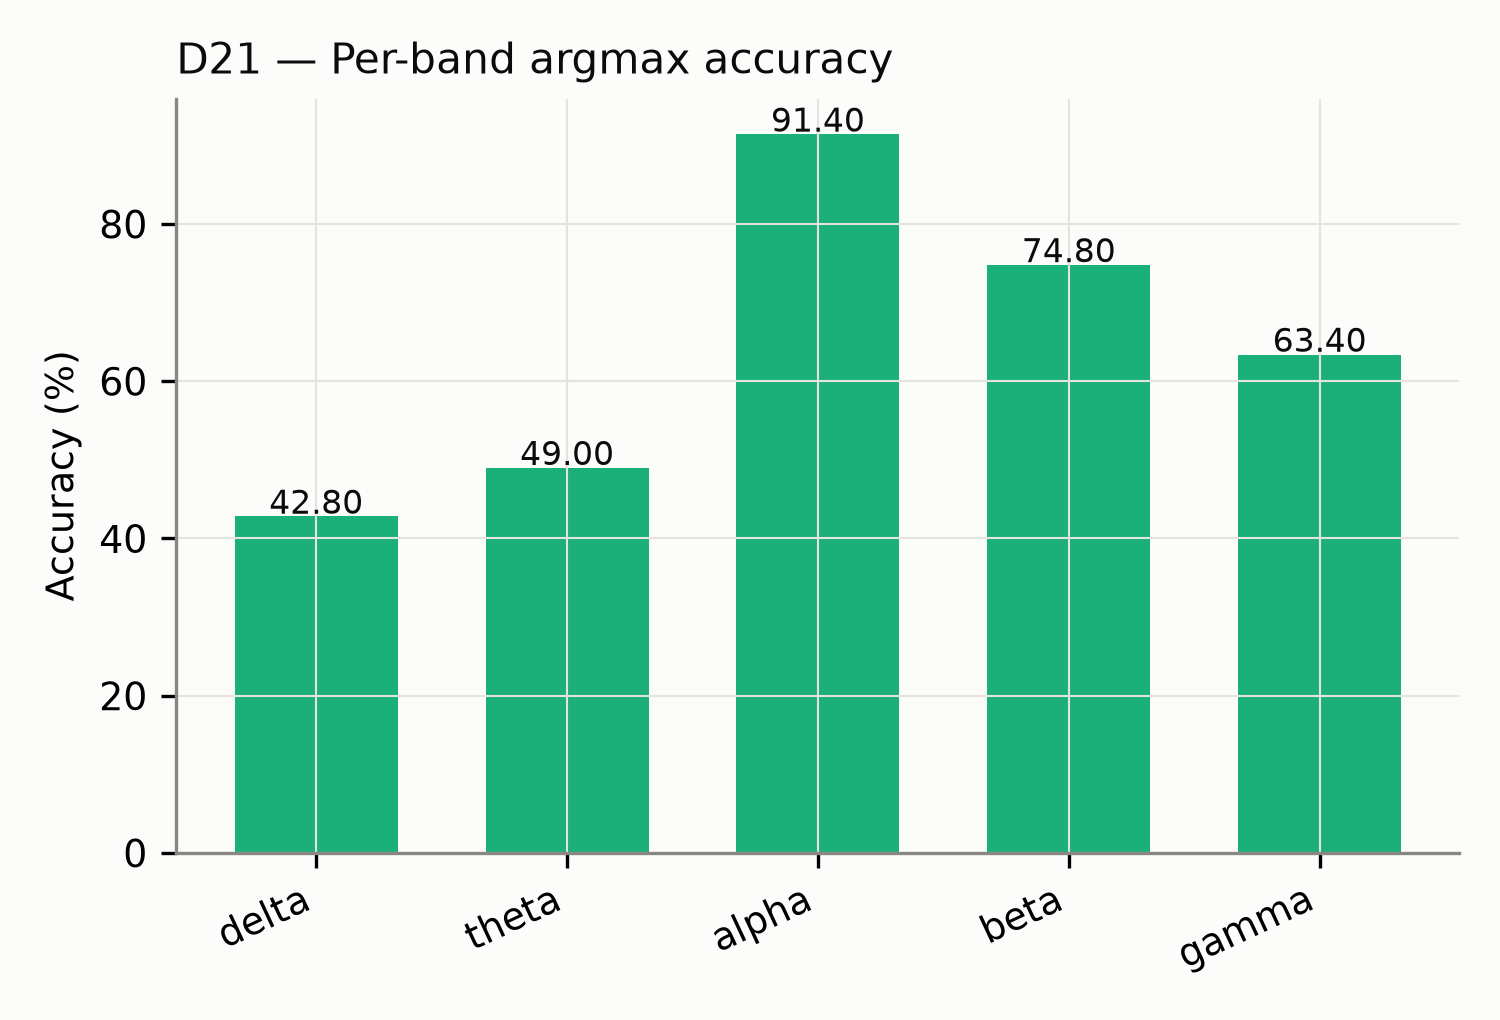
\includegraphics[width=0.49\linewidth]{M3_multiband_fusion/figures/21_individual_band_accuracy.png}\hfill
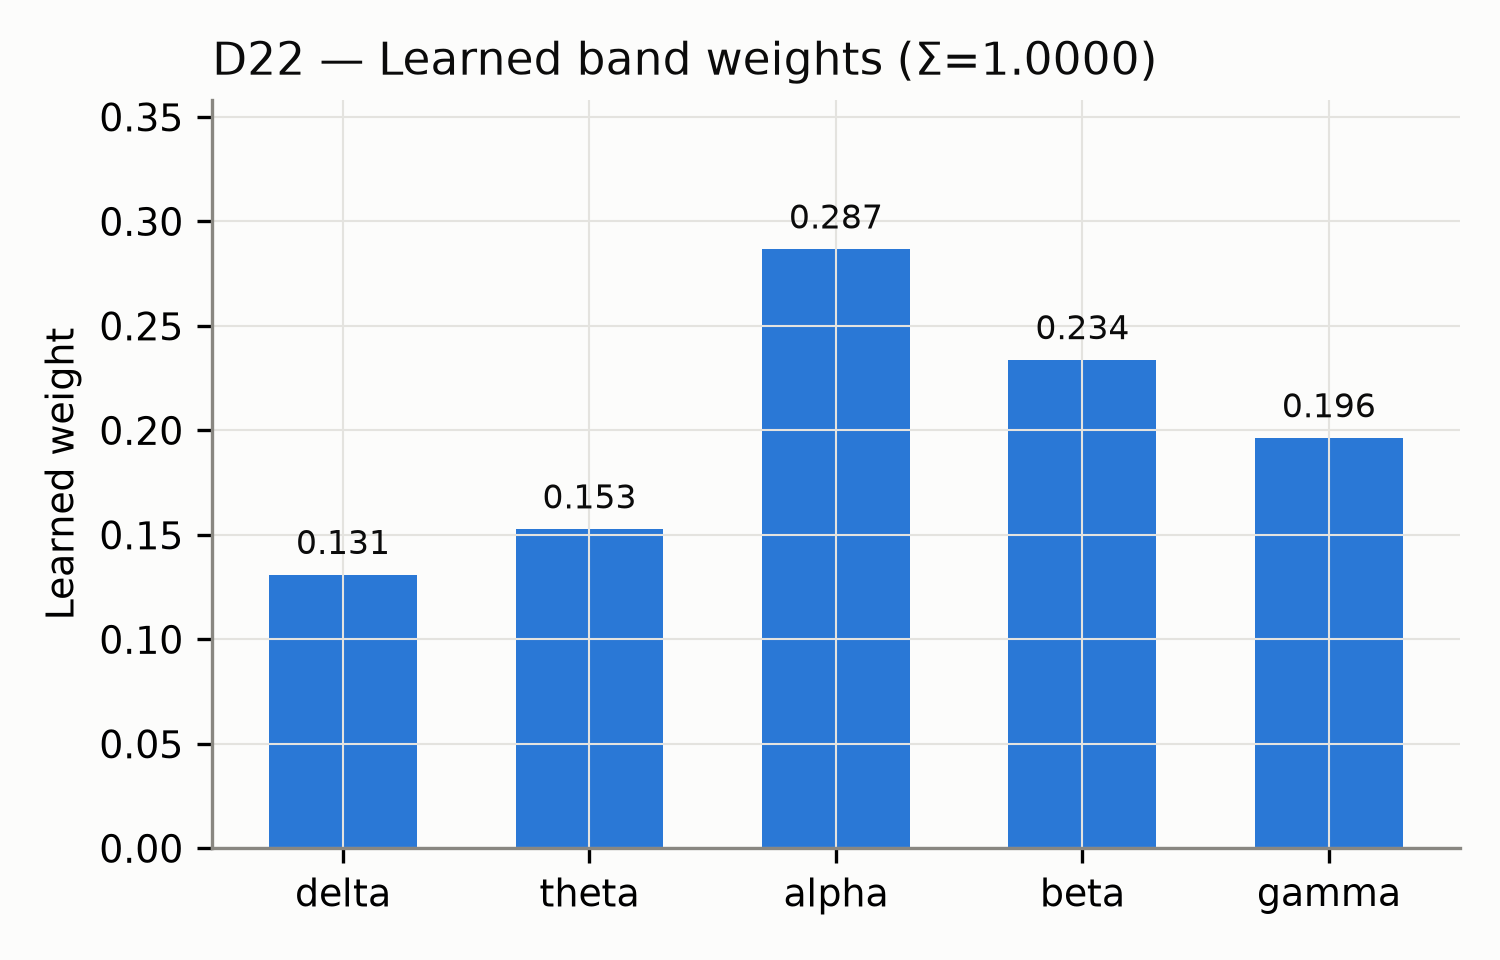
\includegraphics[width=0.49\linewidth]{M3_multiband_fusion/figures/22_learned_band_weights.png}
\caption{Band-specific accuracy (left) and validation-learned fusion weights (right) on \simseed{}}
\label{fig:bands}
\end{figure}

\begin{figure}[t]
\centering
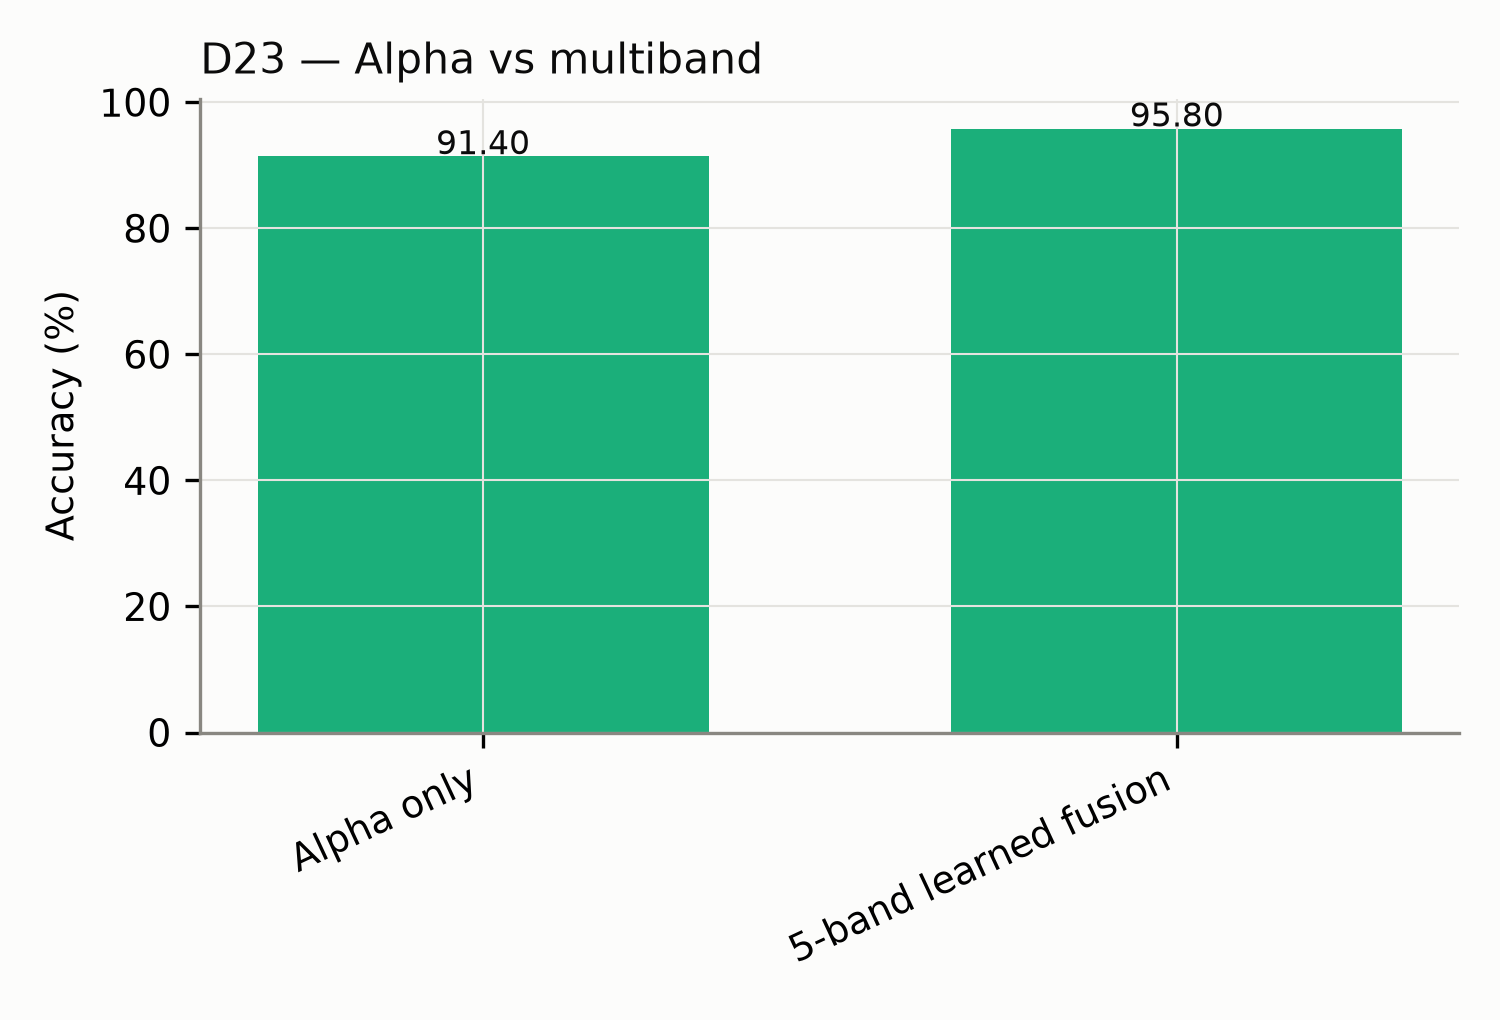
\includegraphics[width=0.49\linewidth]{M3_multiband_fusion/figures/23_alpha_vs_multiband.png}\hfill
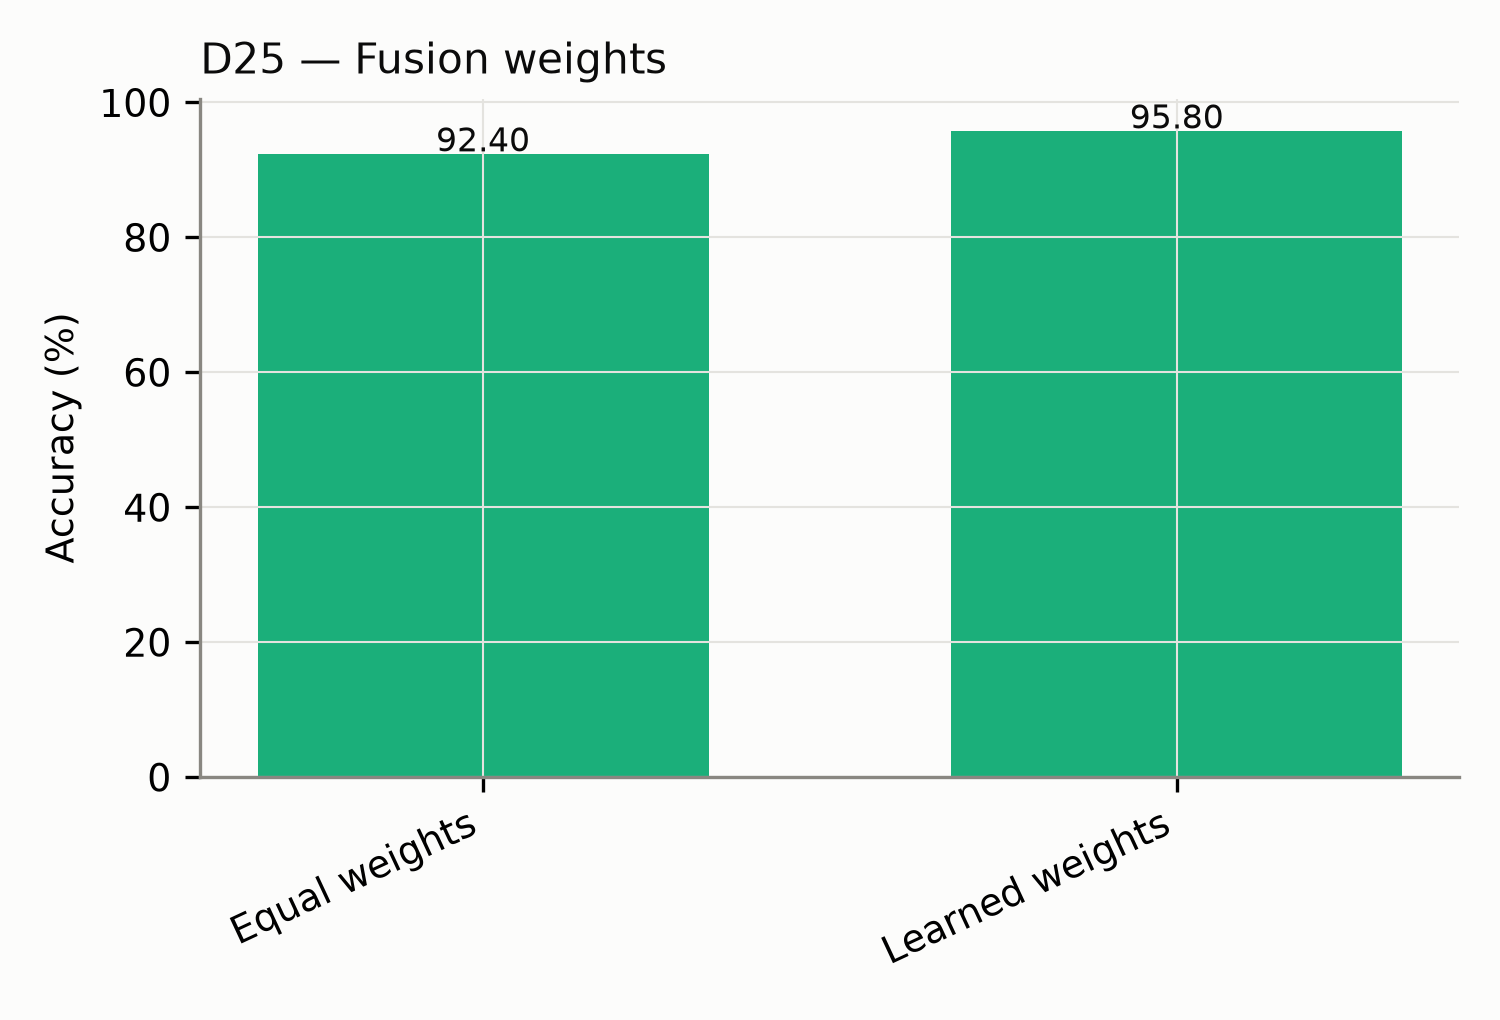
\includegraphics[width=0.49\linewidth]{M3_multiband_fusion/figures/25_equal_vs_learned_fusion.png}
\caption{Alpha band alone versus five-band learned fusion (left) and equal versus learned fusion weights (right) on \simseed{}}
\label{fig:fusecmp}
\end{figure}

\begin{figure}[t]
\centering
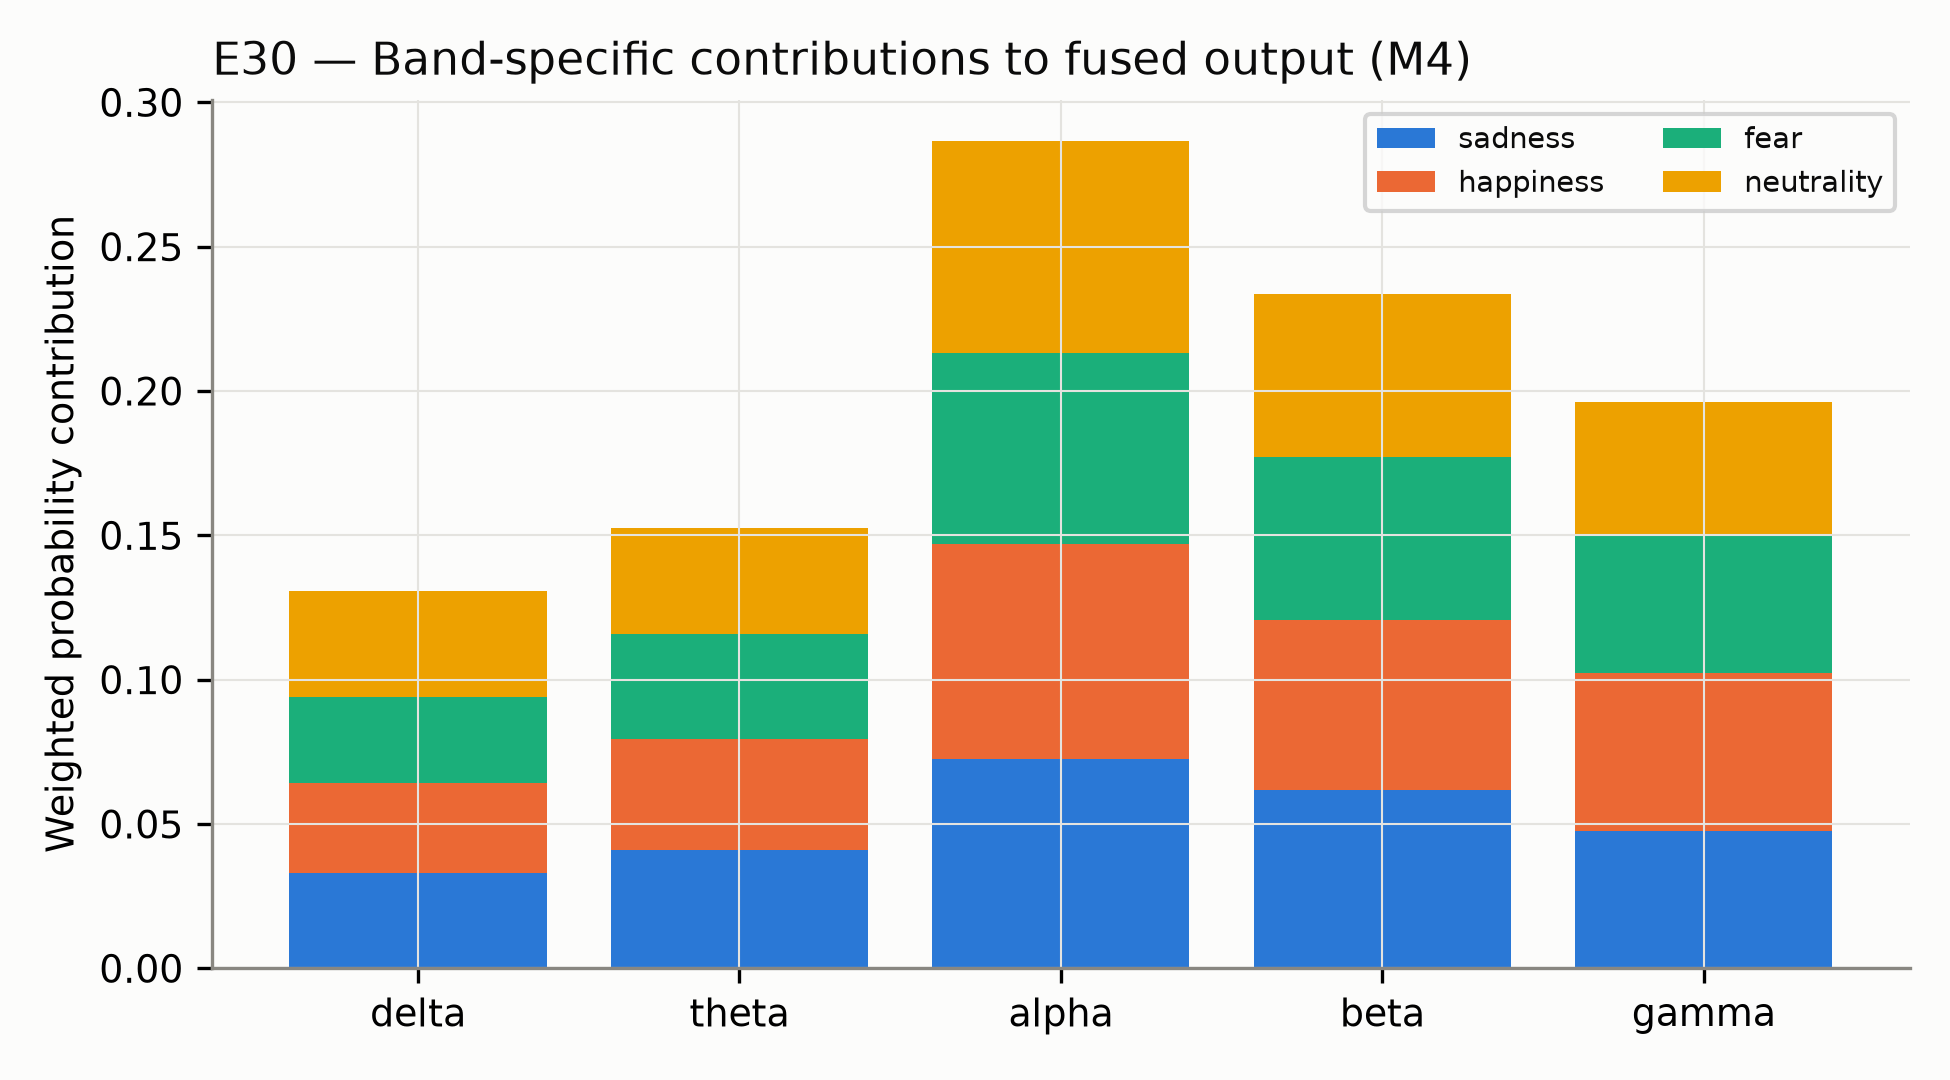
\includegraphics[width=0.8\linewidth]{M4_combined_model/figures/30_m4_band_contributions.png}
\caption{Weighted contribution of each band to the fused class probabilities of M4}
\label{fig:contrib}
\end{figure}

\subsection{Class-wise performance}
Table~\ref{tab:cls} reports per-class precision, recall, F1 and AUC for the baseline and for M4. On \simseed{}, M4 raises the F1 of every class above 95\%, with the largest gain for fear (87.2\% to 95.6\%), the class with the lowest recall under M0. On \simmah{}, fear is the hardest class for M0 (F1 68.8\%) and neutrality for M4 (75.0\%); M4 improves F1 by 3.3--10.7 points for every class. The confusion matrices (Fig.~\ref{fig:cm}) and ROC curves (Fig.~\ref{fig:roc}), pooled over both benchmarks, show the same pattern: after fusion the off-diagonal mass shrinks and all one-versus-rest AUCs reach at least 0.97.

\begin{table}[t]
\caption{Class-wise precision / recall / F1 (\%) / AUC of M0 and M4}
\label{tab:cls}
\scriptsize
\setlength{\tabcolsep}{2.6pt}
\begin{tabular}{@{}l l c c c c@{}}
\toprule
Model & Benchmark & Sadness & Happiness & Fear & Neutrality \\
\midrule
\tabinput generated/tab_per_class.tex 
\bottomrule
\end{tabular}
\end{table}

\begin{figure}[t]
\centering
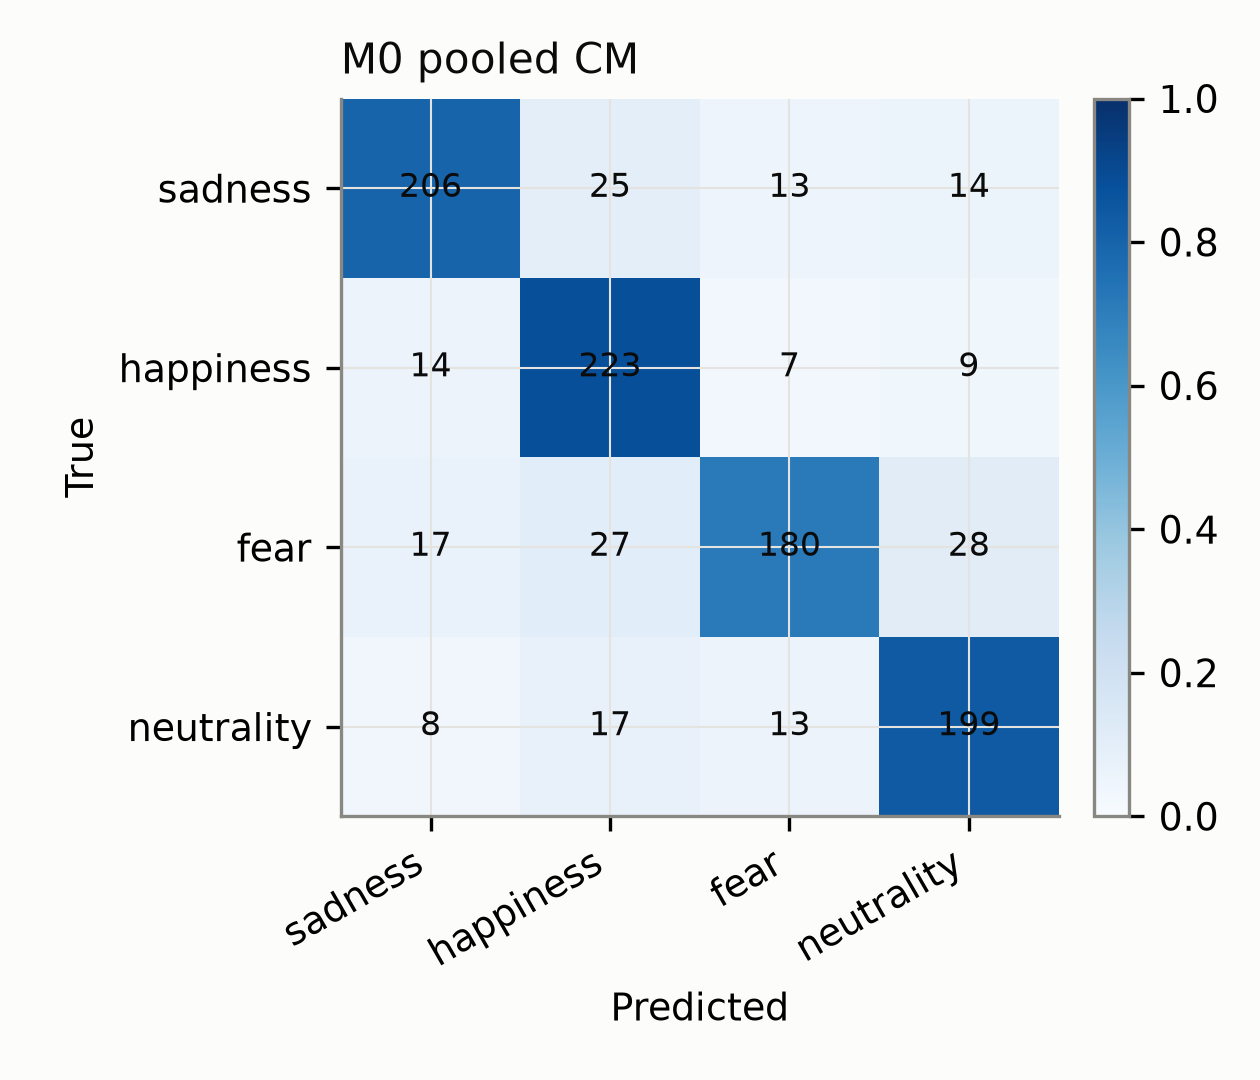
\includegraphics[width=0.49\linewidth]{M0_original/figures/confusion_matrix.png}\hfill
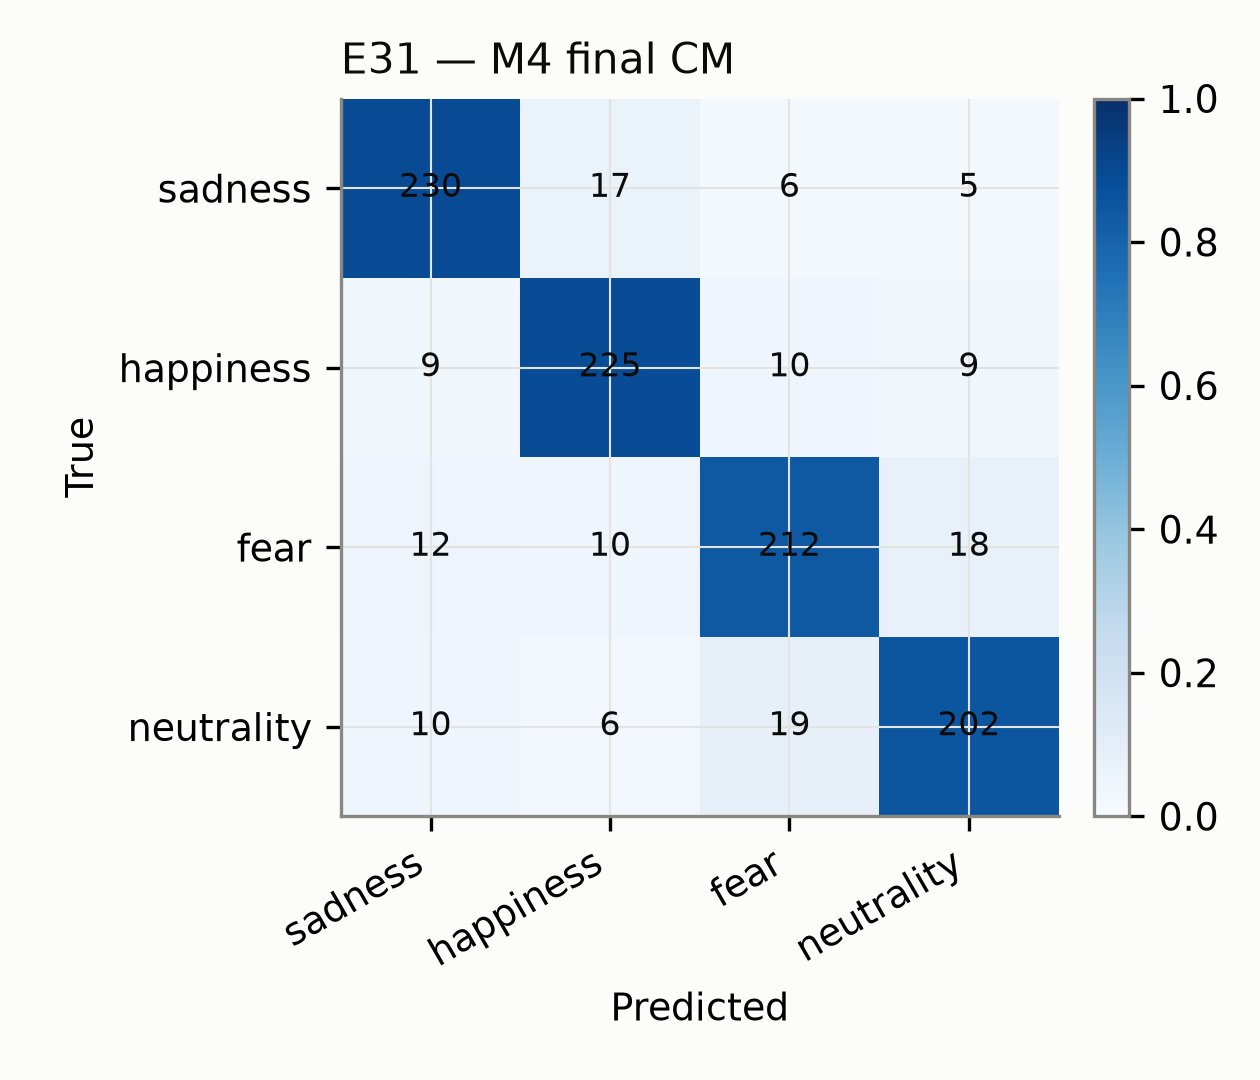
\includegraphics[width=0.49\linewidth]{M4_combined_model/figures/31_final_confusion_matrix.png}
\caption{Confusion matrices of M0 (left) and M4 (right), pooled over \simseed{} and \simmah{} (1000 windows)}
\label{fig:cm}
\end{figure}

\begin{figure}[t]
\centering
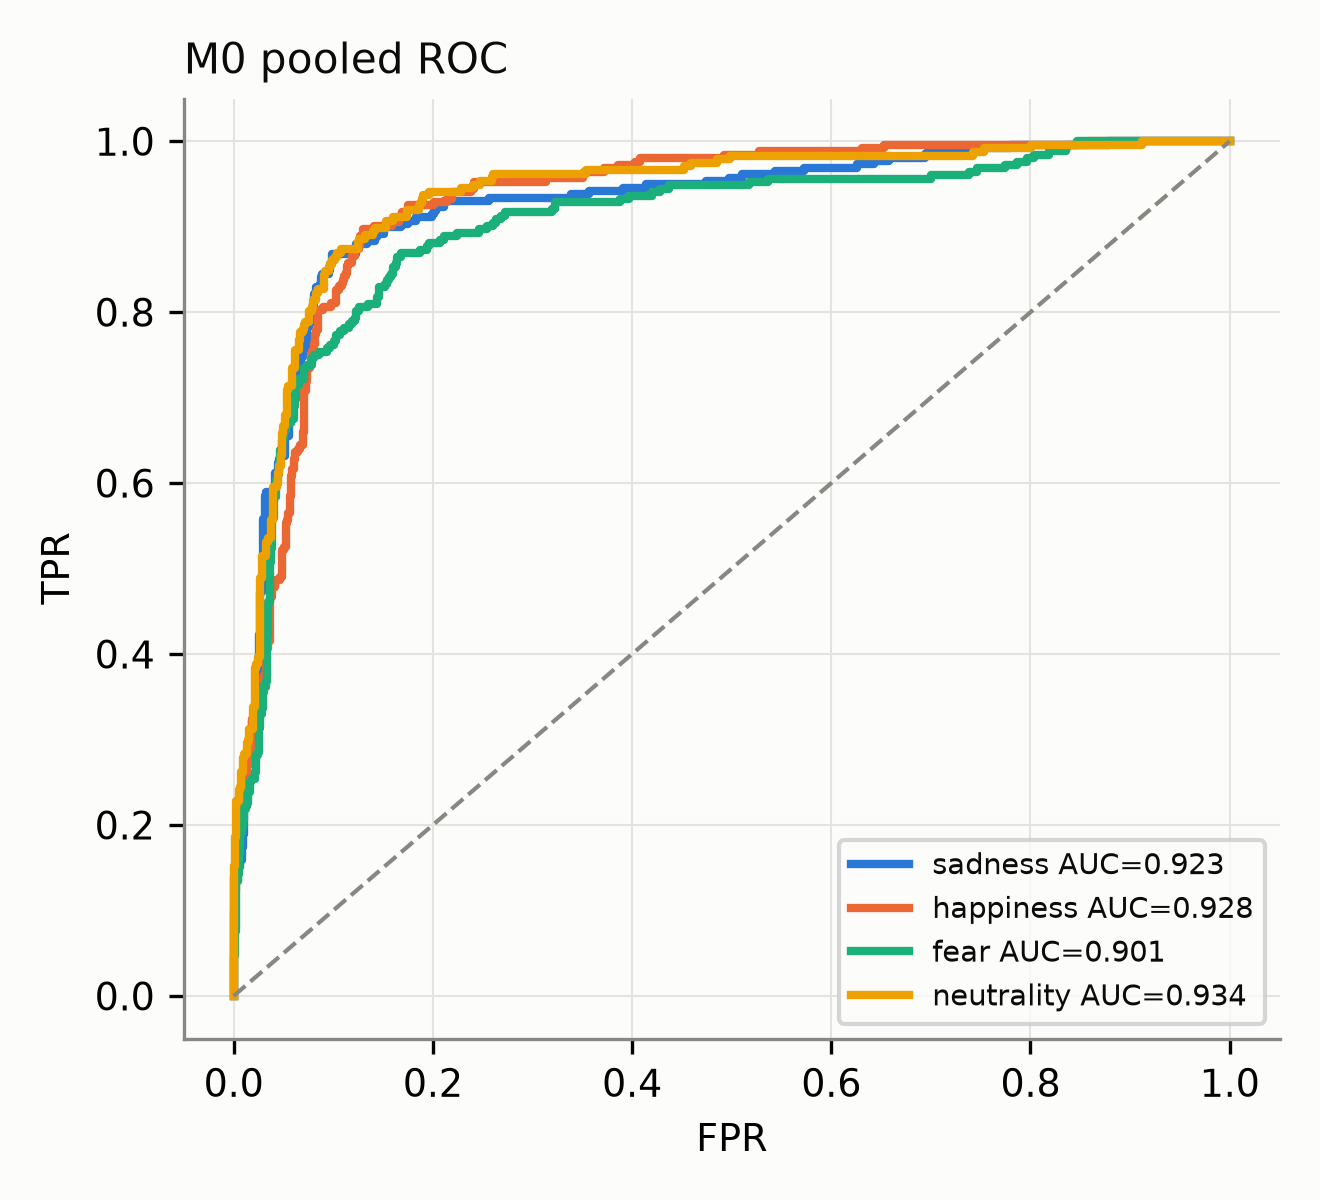
\includegraphics[width=0.49\linewidth]{M0_original/figures/roc_curves.png}\hfill
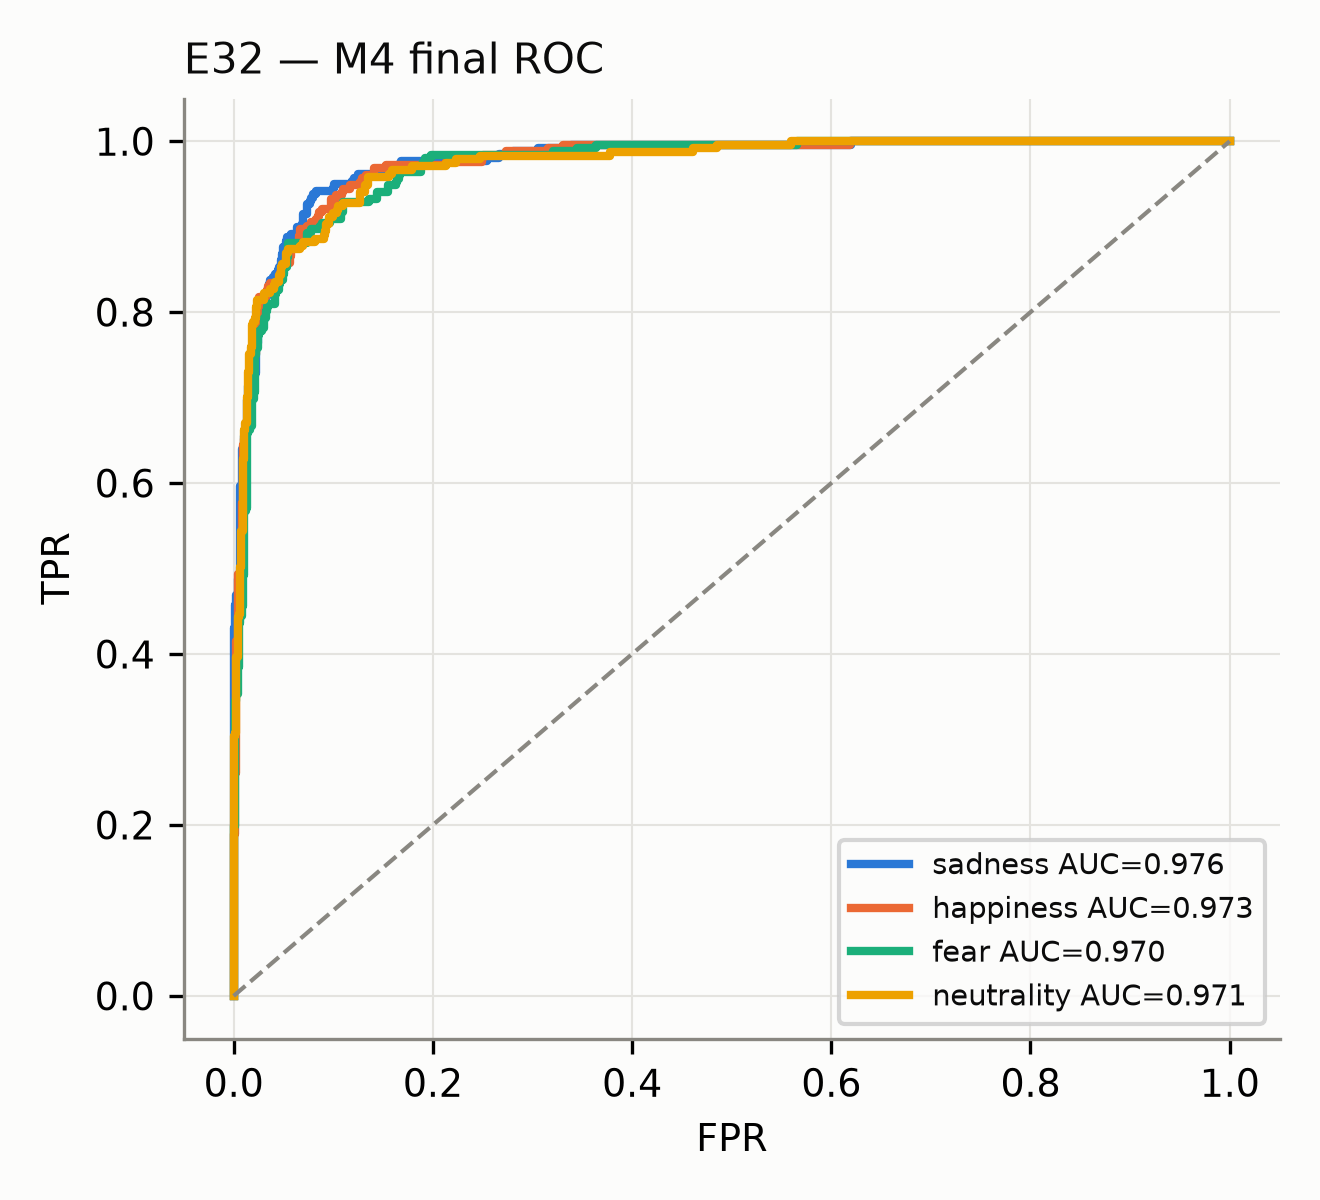
\includegraphics[width=0.49\linewidth]{M4_combined_model/figures/32_final_roc_curves.png}
\caption{One-versus-rest ROC curves of M0 (left) and M4 (right), pooled over both benchmarks}
\label{fig:roc}
\end{figure}

\subsection{Fuzzy rule bases}\label{sec:rules}
Interpretability is the main reason to use an S-FIS. All proposed models keep the rule schema of \cite{FarhadiSedehi2024a}; the gates change \emph{which windows} the rules are learned from, and fusion changes \emph{how the band decisions are combined}, but no rule is hand-written.

\paragraph{Published rules.} Table~\ref{tab:pubrules} lists the ten highest-ranked GA-refined rules of every band on SEED-IV as published in \cite{FarhadiSedehi2024a} (50 rules), and Fig.~\ref{fig:rulemap} gives a compact map of their antecedents and consequents. Happiness is mostly associated with high phase entropy at FP2 combined with low permutation entropy at T7 (e.g.\ A01, B01, G02), sadness with low or medium PhEn-FP2 together with low SampEn-T8 (A05, B05, G05), and fear with medium values of all three inputs (A03, B03, G03). The alpha, beta and gamma bands share most of their top rules, which is consistent with their similar accuracies. Table~\ref{tab:cov} reproduces the coverage and accuracy of the best rule per emotion from the base paper.

\small
\begin{longtable}{@{}c l l l l l@{}}
\caption{GA-refined S-FIS rules of the base paper for SEED-IV (ten per band). Each row reads: IF PhEn-FP2 is \ldots{} AND SampEn-T8 is \ldots{} AND PermEn-T7 is \ldots{} THEN emotion; -- = input absent}\label{tab:pubrules}\\
\toprule
Band & Rule & PhEn-FP2 & SampEn-T8 & PermEn-T7 & THEN \\
\midrule
\endfirsthead
\multicolumn{6}{@{}l}{\footnotesize\textbf{Table \thetable} (continued)}\\
\toprule
Band & Rule & PhEn-FP2 & SampEn-T8 & PermEn-T7 & THEN \\
\midrule
\endhead
\bottomrule
\multicolumn{6}{@{}p{0.95\linewidth}@{}}{\footnotesize $^{\dagger}$Rule G01 uses permutation entropy at FP2 in the source; the spelling is kept.}
\endlastfoot
\tabinput generated/tab_published_rules.tex 
\end{longtable}
\normalsize

\begin{figure}[t]
\centering
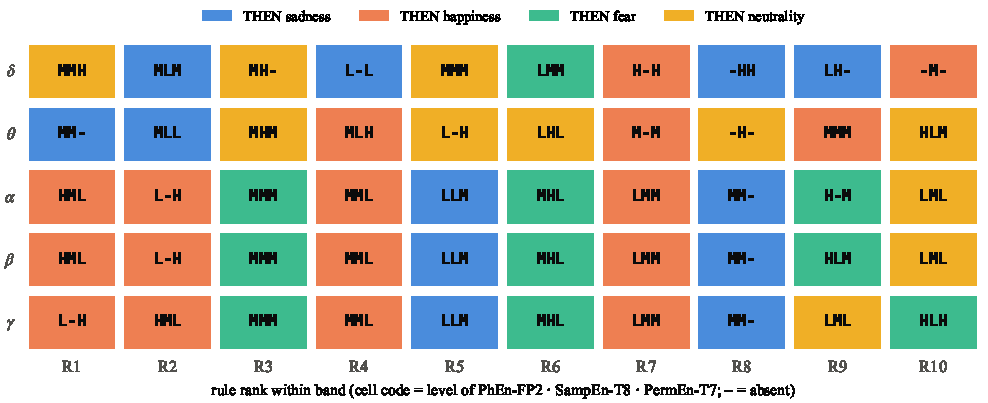
\includegraphics[width=\linewidth]{fig10_rule_map.pdf}
\caption{Map of the 50 published rules: rows are frequency bands, columns rule ranks; the cell code gives the levels (L/M/H) of PhEn-FP2, SampEn-T8 and PermEn-T7 and the colour the consequent emotion}
\label{fig:rulemap}
\end{figure}

\begin{table}[t]
\caption{Coverage and accuracy of the most discriminative rules per emotion, as reported in \cite{FarhadiSedehi2024a} (spellings as in the source)}
\label{tab:cov}
\scriptsize
\setlength{\tabcolsep}{3pt}
\begin{tabularx}{\linewidth}{@{}r l X r r@{}}
\toprule
\# & Emotion & Rule antecedent & Cov. (\%) & Acc. (\%) \\
\midrule
\tabinput generated/tab_rule_coverage.tex 
\bottomrule
\end{tabularx}
\end{table}

\paragraph{Rules mined by our implementation.} To verify that the implementation mines rules from raw signals, the complete pipeline was run on the synthetic signal-level set (Table~\ref{tab:data}) with three MFs per input. The eye-feature mRMR selected the mean fixation duration as gate feature, and the hard gate kept 144 of 384 windows. Table~\ref{tab:minedsum} summarises the per-band classifiers and Table~\ref{tab:mined} lists the ten highest-ranked rules of the two best bands, ranked by coverage $\times$ accuracy $\times$ weight. The GA pruned the lookup-table rule base by 24--31\% (e.g.\ 18.4 to 13.2 rules in beta) while changing accuracy by between $-4.2$ (alpha) and $+2.0$ (theta) points, and converged within 17--29 generations (Fig.~\ref{fig:ga}). The accuracies (25--49\%) are much lower than on the simulation benchmarks because this set has only four participants and weak class structure; they confirm that the pipeline works, not how well it would perform on real EEG. Several mined rules are compact and specific---for example, beta rule 3 (``SymbEn-T7 low $\wedge$ SymbEn-FP2 medium $\wedge$ SymbEn-T8 low $\Rightarrow$ sad'') covers 14\% of the windows with 95.6\% accuracy---which illustrates the kind of readable evidence an S-FIS provides.

\begin{table}[t]
\caption{Pipeline run on the synthetic signal-level set: accuracy (\%, mean $\pm$ s.d. over 5 folds), accuracy of the lookup table before GA, macro-F1, macro-AUC, mean rule count before and after GA, and GA generations}
\label{tab:minedsum}
\scriptsize
\setlength{\tabcolsep}{3.4pt}
\begin{tabular*}{\linewidth}{@{\extracolsep{\fill}}l c r r r r r r@{}}
\toprule
Band & Acc. & Lookup acc. & F1 & AUC & Rules (LT) & Rules (GA) & Gen. \\
\midrule
\tabinput generated/tab_mined_summary.tex 
\bottomrule
\end{tabular*}
\end{table}

\begin{table}[t]
\caption{Top-ten rules mined by the S-FIS--GA on the synthetic signal-level set for the alpha and beta bands. Cov.: share of windows that fire the rule; Acc.: accuracy on those windows}
\label{tab:mined}
\scriptsize
\setlength{\tabcolsep}{2.6pt}
\begin{tabularx}{\linewidth}{@{}c r X l r r@{}}
\toprule
Band & \# & IF (antecedent) & THEN & Cov. (\%) & Acc. (\%) \\
\midrule
\tabinput generated/tab_mined_rules.tex 
\bottomrule
\end{tabularx}
\end{table}

\begin{figure}[t]
\centering
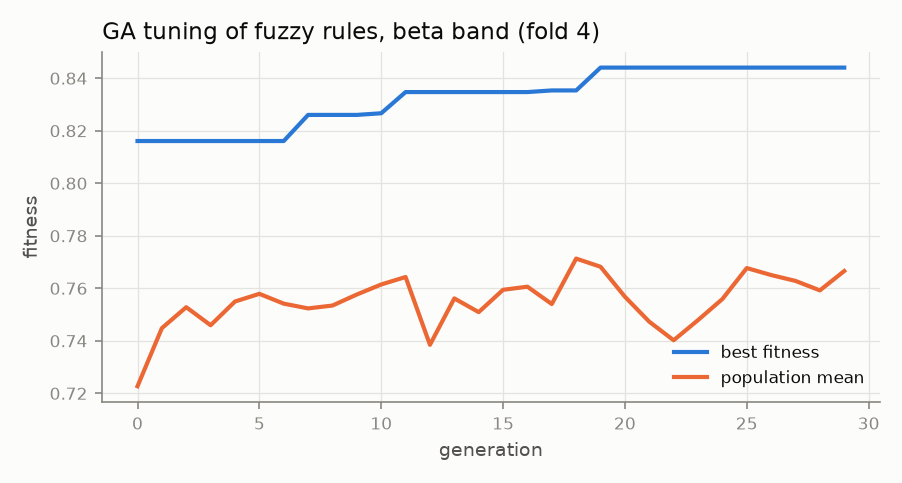
\includegraphics[width=0.78\linewidth]{ga_curve_beta.png}
\caption{GA refinement of the beta-band rule base (best fold): best and mean fitness (Eq.~\ref{eq:fitness}) per generation}
\label{fig:ga}
\end{figure}

\subsection{Relation to the base paper}
The base paper reports 94.42\% (alpha), 93.02\% (beta) and 89.80\% (gamma) on SEED-IV and 85.20\%, 82.92\% and 79.05\% on MAHNOB-HCI \cite{FarhadiSedehi2024a}. Our benchmarks were calibrated to this scale, so the absolute accuracies of Table~\ref{tab:main} are a consequence of the calibration and must not be read as improvements over, or reproductions of, these numbers. What the simulation does establish is the \emph{relative} behaviour of the design choices under a common protocol with paired tests: (i) late fusion of band-specific fuzzy classifiers with validation-learned weights is the most reliable improvement; (ii) subject-specific baseline correction of the gate signal is more useful than softening the threshold; and (iii) once bands are fused, the choice of gate matters little.

\subsection{Limitations}
The main limitation is that the M0--M4 comparison uses synthetic benchmarks in which band posteriors are generated rather than produced by trained S-FIS, so effects that depend on real EEG---for example, how gate weights change the selected entropy features---are not captured. In the benchmark runs, M0 and M1 are scored on different single-band heads, which confounds their comparison. The DWT bands of our implementation are dyadic and differ slightly from the ranges stated in the base paper. Window-level five-fold cross-validation, used here to match the base paper, is optimistic for EEG because windows of one trial are correlated \cite{Li2021,Kukhilava2025}; trial-wise or leave-one-subject-out validation is preferable on real data. Finally, the pupil response depends on luminance, which the simulation does not model \cite{Raiturkar2016}.

% ===================================================================== 6
\section{Conclusion}\label{sec:conclusion}
This paper re-implemented the eye-tracking-gated Sugeno fuzzy EEG emotion recogniser of \cite{FarhadiSedehi2024a} and extended it with a fuzzy eye gate, an adaptive temporal gate and validation-weighted multi-band fusion. In a controlled simulation study calibrated to SEED-IV and MAHNOB-HCI, the combined model reached 96.00\% accuracy on \simseed{} and multi-band fusion reached 79.00\% on \simmah{}, improving on the hard-gated single-band baseline by 4.6 and 8.8 points with significant paired tests. Fusion was the most consistent source of improvement, baseline-corrected gating helped mainly on the harder benchmark, and a fuzzy gate alone did not improve classification. The complete fuzzy rule bases, from the base paper and from our own GA, are reported for interpretability.

In future, we intend to obtain licensed access to SEED-IV and MAHNOB-HCI and evaluate M0--M4 with trained S-FIS on real recordings under subject-independent protocols, replace the window-weighting gate by a fuzzy gate learned jointly with the classifier, and model luminance explicitly in the pupil baseline. A causal smoothing variant is already implemented and will allow online, real-time operation on wearable EEG--eye-tracking hardware.

\vspace{10pt}
{\small
\noindent{\sffamily\bfseries Author contributions}\enspace Both authors contributed to the design and implementation of the system, the experiments and the preparation of the manuscript. Both authors read and approved the final manuscript.

\vspace{4pt}
\noindent{\sffamily\bfseries Funding}\enspace The authors did not receive support from any organization for the submitted work.

\vspace{4pt}
\noindent{\sffamily\bfseries Data availability}\enspace No new human-subject data were collected. The synthetic benchmarks, prediction files, generator settings and the code that produces every table and figure are available from the authors on reasonable request. SEED-IV and MAHNOB-HCI can be requested from their providers under their licence terms.

\vspace{8pt}
\noindent{\sffamily\bfseries\large Declarations}

\vspace{4pt}
\noindent{\sffamily\bfseries Conflict of interest}\enspace The authors have no conflict of interest to declare that is relevant to the content of this article.

\vspace{4pt}
\noindent{\sffamily\bfseries Ethical approval}\enspace Not applicable; the study uses only synthetic data.

\vspace{4pt}
\noindent{\sffamily\bfseries Consent for publication}\enspace All authors consent to the publication of this work.
}

% ===================================================================== refs
\renewcommand{\refname}{\sffamily\bfseries\large References}
{\footnotesize
\setlength{\itemsep}{0pt}
\begin{thebibliography}{99}
\bibitem{Alarcao2019} Alarc\~ao SM, Fonseca MJ (2019) Emotions recognition using EEG signals: a survey. IEEE Trans Affect Comput 10(3):374--393. \url{https://doi.org/10.1109/TAFFC.2017.2714671}

\bibitem{Arevalo2020} Arevalo J, Solorio T, Montes-y-G\'omez M, Gonz\'alez FA (2020) Gated multimodal networks. Neural Comput Appl 32(14):10209--10228. \url{https://doi.org/10.1007/s00521-019-04559-1}

\bibitem{Bandt2002} Bandt C, Pompe B (2002) Permutation entropy: a natural complexity measure for time series. Phys Rev Lett 88(17):174102. \url{https://doi.org/10.1103/PhysRevLett.88.174102}

\bibitem{Bradley2008} Bradley MM, Miccoli L, Escrig MA, Lang PJ (2008) The pupil as a measure of emotional arousal and autonomic activation. Psychophysiology 45(4):602--607. \url{https://doi.org/10.1111/j.1469-8986.2008.00654.x}

\bibitem{ChoKim1995} Cho SB, Kim JH (1995) Combining multiple neural networks by fuzzy integral for robust classification. IEEE Trans Syst Man Cybern 25(2):380--384. \url{https://doi.org/10.1109/21.364825}

\bibitem{Demsar2006} Dem\v{s}ar J (2006) Statistical comparisons of classifiers over multiple data sets. J Mach Learn Res 7:1--30

\bibitem{Duan2013} Duan RN, Zhu JY, Lu BL (2013) Differential entropy feature for EEG-based emotion classification. In: 6th Int IEEE/EMBS Conf Neural Engineering (NER), pp 81--84. \url{https://doi.org/10.1109/NER.2013.6695876}

\bibitem{FarhadiSedehi2024a} Farhadi Sedehi J, Jafarnia Dabanloo N, Maghooli K, Sheikhani A (2024) Recognition of emotional categories using mined fuzzy rules from electroencephalogram signals with gated eye track data approach. IEEE Access 12:118122--118140. \url{https://doi.org/10.1109/ACCESS.2024.3430934}

\bibitem{FarhadiSedehi2024b} Farhadi Sedehi J, Jafarnia Dabanloo N, Maghooli K, Sheikhani A (2024) Multimodal insights into Granger causality connectivity: integrating physiological signals and gated eye-tracking data for emotion recognition using convolutional neural network. Heliyon 10(16):e36411. \url{https://doi.org/10.1016/j.heliyon.2024.e36411}

\bibitem{Fu2023} Fu B, Gu C, Fu M, Xia Y, Liu Y (2023) A novel feature fusion network for multimodal emotion recognition from EEG and eye movement signals. Front Neurosci 17:1234162. \url{https://doi.org/10.3389/fnins.2023.1234162}

\bibitem{Jacobs1991} Jacobs RA, Jordan MI, Nowlan SJ, Hinton GE (1991) Adaptive mixtures of local experts. Neural Comput 3(1):79--87. \url{https://doi.org/10.1162/neco.1991.3.1.79}

\bibitem{Jang1993} Jang JSR (1993) ANFIS: adaptive-network-based fuzzy inference system. IEEE Trans Syst Man Cybern 23(3):665--685. \url{https://doi.org/10.1109/21.256541}

\bibitem{Jenke2014} Jenke R, Peer A, Buss M (2014) Feature extraction and selection for emotion recognition from EEG. IEEE Trans Affect Comput 5(3):327--339. \url{https://doi.org/10.1109/TAFFC.2014.2339834}

\bibitem{Kaya2024} Kaya \"U, Akay D, \c{S}eng\"ul Ayan S (2024) EEG-based emotion recognition in neuromarketing using fuzzy linguistic summarization. IEEE Trans Fuzzy Syst 32(8):4248--4259. \url{https://doi.org/10.1109/TFUZZ.2024.3392495}

\bibitem{Kittler1998} Kittler J, Hatef M, Duin RPW, Matas J (1998) On combining classifiers. IEEE Trans Pattern Anal Mach Intell 20(3):226--239. \url{https://doi.org/10.1109/34.667881}

\bibitem{Kret2019} Kret ME, Sjak-Shie EE (2019) Preprocessing pupil size data: guidelines and code. Behav Res Methods 51(3):1336--1342. \url{https://doi.org/10.3758/s13428-018-1075-y}

\bibitem{Kukhilava2025} Kukhilava N, Tsmindashvili T, Kalandadze R, et al (2025) Evaluation in EEG emotion recognition: state-of-the-art review and unified framework. arXiv:2505.18175 (preprint)

\bibitem{Li2021} Li R, Johansen JS, Ahmed H, Ilyevsky TV, Wilbur RB, Bharadwaj HM, Siskind JM (2021) The perils and pitfalls of block design for EEG classification experiments. IEEE Trans Pattern Anal Mach Intell 43(1):316--333. \url{https://doi.org/10.1109/TPAMI.2020.2973153}

\bibitem{Lim2020} Lim JZ, Mountstephens J, Teo J (2020) Emotion recognition using eye-tracking: taxonomy, review and current challenges. Sensors 20(8):2384. \url{https://doi.org/10.3390/s20082384}

\bibitem{LinWang2002} Lin CF, Wang SD (2002) Fuzzy support vector machines. IEEE Trans Neural Netw 13(2):464--471. \url{https://doi.org/10.1109/72.991432}

\bibitem{Liu2022} Liu W, Qiu JL, Zheng WL, Lu BL (2022) Comparing recognition performance and robustness of multimodal deep learning models for multimodal emotion recognition. IEEE Trans Cogn Dev Syst 14(2):715--729. \url{https://doi.org/10.1109/TCDS.2021.3071170}

\bibitem{Lu2015} Lu Y, Zheng WL, Li B, Lu BL (2015) Combining eye movements and EEG to enhance emotion recognition. In: Proc 24th Int Joint Conf Artificial Intelligence (IJCAI), pp 1170--1175

\bibitem{Mallat1989} Mallat SG (1989) A theory for multiresolution signal decomposition: the wavelet representation. IEEE Trans Pattern Anal Mach Intell 11(7):674--693. \url{https://doi.org/10.1109/34.192463}

\bibitem{Mathot2018} Math\^ot S (2018) Pupillometry: psychology, physiology, and function. J Cogn 1(1):16. \url{https://doi.org/10.5334/joc.18}

\bibitem{Matiko2014} Matiko JW, Beeby SP, Tudor J (2014) Fuzzy logic based emotion classification. In: Proc IEEE Int Conf Acoustics, Speech and Signal Processing (ICASSP), pp 4389--4393. \url{https://doi.org/10.1109/ICASSP.2014.6854431}

\bibitem{McNemar1947} McNemar Q (1947) Note on the sampling error of the difference between correlated proportions or percentages. Psychometrika 12(2):153--157. \url{https://doi.org/10.1007/BF02295996}

\bibitem{Murugappan2010} Murugappan M, Ramachandran N, Sazali Y (2010) Classification of human emotion from EEG using discrete wavelet transform. J Biomed Sci Eng 3(4):390--396. \url{https://doi.org/10.4236/jbise.2010.34054}

\bibitem{Nandakumar2008} Nandakumar K, Chen Y, Dass SC, Jain AK (2008) Likelihood ratio-based biometric score fusion. IEEE Trans Pattern Anal Mach Intell 30(2):342--347. \url{https://doi.org/10.1109/TPAMI.2007.70796}

\bibitem{Partala2003} Partala T, Surakka V (2003) Pupil size variation as an indication of affective processing. Int J Hum-Comput Stud 59(1--2):185--198. \url{https://doi.org/10.1016/S1071-5819(03)00017-X}

\bibitem{Peng2005} Peng H, Long F, Ding C (2005) Feature selection based on mutual information criteria of max-dependency, max-relevance, and min-redundancy. IEEE Trans Pattern Anal Mach Intell 27(8):1226--1238. \url{https://doi.org/10.1109/TPAMI.2005.159}

\bibitem{Raiturkar2016} Raiturkar P, Kleinsmith A, Keil A, Banerjee A, Jain E (2016) Decoupling light reflex from pupillary dilation to measure emotional arousal in videos. In: Proc ACM Symp Applied Perception (SAP), pp 89--96. \url{https://doi.org/10.1145/2931002.2931009}

\bibitem{Richman2000} Richman JS, Moorman JR (2000) Physiological time-series analysis using approximate entropy and sample entropy. Am J Physiol Heart Circ Physiol 278(6):H2039--H2049. \url{https://doi.org/10.1152/ajpheart.2000.278.6.H2039}

\bibitem{Rohila2019} Rohila A, Sharma A (2019) Phase entropy: a new complexity measure for heart rate variability. Physiol Meas 40(10):105006. \url{https://doi.org/10.1088/1361-6579/ab499e}

\bibitem{Soleymani2012db} Soleymani M, Lichtenauer J, Pun T, Pantic M (2012) A multimodal database for affect recognition and implicit tagging. IEEE Trans Affect Comput 3(1):42--55. \url{https://doi.org/10.1109/T-AFFC.2011.25}

\bibitem{TakagiSugeno1985} Takagi T, Sugeno M (1985) Fuzzy identification of systems and its applications to modeling and control. IEEE Trans Syst Man Cybern SMC-15(1):116--132. \url{https://doi.org/10.1109/TSMC.1985.6313399}

\bibitem{WangMendel1992} Wang LX, Mendel JM (1992) Generating fuzzy rules by learning from examples. IEEE Trans Syst Man Cybern 22(6):1414--1427. \url{https://doi.org/10.1109/21.199466}

\bibitem{Zadeh1965} Zadeh LA (1965) Fuzzy sets. Inf Control 8(3):338--353. \url{https://doi.org/10.1016/S0019-9958(65)90241-X}

\bibitem{Zebrowski2000} \.Zebrowski JJ, Pop\l awska W, Baranowski R, Buchner T (2000) Symbolic dynamics and complexity in a physiological time series. Chaos Solitons Fractals 11(7):1061--1075. \url{https://doi.org/10.1016/S0960-0779(99)00004-1}

\bibitem{ZhengDong2014} Zheng WL, Dong BN, Lu BL (2014) Multimodal emotion recognition using EEG and eye tracking data. In: Proc 36th Annu Int Conf IEEE Eng Med Biol Soc (EMBC), pp 5040--5043. \url{https://doi.org/10.1109/EMBC.2014.6944757}

\bibitem{Zheng2019} Zheng WL, Liu W, Lu Y, Lu BL, Cichocki A (2019) EmotionMeter: a multimodal framework for recognizing human emotions. IEEE Trans Cybern 49(3):1110--1122. \url{https://doi.org/10.1109/TCYB.2018.2797176}

\bibitem{ZhengLu2015} Zheng WL, Lu BL (2015) Investigating critical frequency bands and channels for EEG-based emotion recognition with deep neural networks. IEEE Trans Auton Ment Dev 7(3):162--175. \url{https://doi.org/10.1109/TAMD.2015.2431497}

\end{thebibliography}

}

\end{document}
